\PassOptionsToPackage{table}{xcolor}

\documentclass[sigconf]{acmart}

\usepackage[colorlinks=true,
            linkcolor=blue,
            urlcolor=blue,
            citecolor=blue]{hyperref}

\usepackage{tikz}

\newcommand{\ExternalLink}{%
    \tikz[x=1.2ex, y=1.2ex, baseline=-0.05ex]{% 
        \begin{scope}[x=1ex, y=1ex]
            \clip (-0.1,-0.1) 
                --++ (-0, 1.2) 
                --++ (0.6, 0) 
                --++ (0, -0.6) 
                --++ (0.6, 0) 
                --++ (0, -1);
            \path[draw, 
                line width = 0.5, 
                rounded corners=0.5] 
                (0,0) rectangle (1,1);
        \end{scope}
        \path[draw, line width = 0.5] (0.5, 0.5) 
            -- (1, 1);
        \path[draw, line width = 0.5] (0.6, 1) 
            -- (1, 1) -- (1, 0.6);
        }
    }
    
\usepackage{caption}
\usepackage[T1]{fontenc}
\usepackage[latin1]{inputenc}
\usepackage{fancyvrb}
\usepackage{subcaption}
\usepackage{graphicx}

%enumeration subnumbers


\renewcommand{\labelenumi}{\arabic{enumi}.} 
\renewcommand{\labelenumii}{\arabic{enumi}.\arabic{enumii}}


\usepackage{todonotes}
\newcommand{\TODO}[1]{\todo[inline]{#1}}
\newcommand{\NOTE}[1]{\textcolor{red}{[NOTE: #1]}}
\newcommand{\FILE}[1]{\todo[inline,color=green!20]{File: #1}}

\newcommand{\OK}{+}
\newcommand{\OP}{o}
%\newcommand{\NA}{n/a}
\newcommand{\NA}{-}

\definecolor{lightgray}{gray}{0.94}
\let\oldtabular\tabular
\let\endoldtabular\endtabular
\renewenvironment{tabular}{\rowcolors{2}{lightgray}{white}\oldtabular}{\endoldtabular}

\setcopyright{none}
\copyrightyear{2022}
\acmYear{2022}
\acmDOI{}

\acmConference[White Paper]{White paper produced by the NIST Public Working Group on Big Data}{White paper produced by the NIST Public Working Group on Big Data}{Washington, D.C.}
\acmBooktitle{White paper produced by the NIST Public Working Group on Big Data, Washington, D.C.}
\acmPrice{}
\acmISBN{}
%%\citestyle{acmauthoryear}

\makeatletter
\def\@copyrightspace{\relax}
\makeatother

\begin{document}

\title{Reusable Hybrid and Multi-Cloud Analytics Service Framework}

\author{Gregor von Laszewski}
\email{laszewski@gmail.com}
\orcid{0000-0001-9558-179X}
\affiliation{%
  \institution{University of Virginia}
  \streetaddress{Biocomplexity Institute\\
                Town Center Four\\
                994 Research Park Boulevard}
  \city{Charlottesville}
  \state{VA}
  \country{USA}
}

\author{Wo Chang}
\email{laszewski@gmail.com}
\orcid{0000-0001-9558-179X}
\affiliation{%
  \institution{University of Virginia}
  \streetaddress{Biocomplexity Institute\\
                Town Center Four\\
                994 Research Park Boulevard}
  \city{Charlottesville}
  \state{VA}
  \country{USA}
}

\author{Geoffrey C. Fox}
\email{gcfexchange@gmail.com}
\affiliation{%
  \institution{University of Virginia}
  \streetaddress{Biocomplexity Institute\\
                Town Center Four\\
                994 Research Park Boulevard}
  \city{Charlottesville}
  \state{VA}
  \country{USA}
}

\author{Russel Reinsch}
\email{laszewski@gmail.com}
\orcid{0000-0001-9558-179X}
\affiliation{%
  \institution{University of Virginia}
  \streetaddress{Biocomplexity Institute\\
                Town Center Four\\
                994 Research Park Boulevard}
  \city{Charlottesville}
  \state{VA}
  \country{USA}
}

\author{Ali ...}
\email{laszewski@gmail.com}
\orcid{0000-0001-9558-179X}
\affiliation{%
  \institution{University of Virginia}
  \streetaddress{Biocomplexity Institute\\
                Town Center Four\\
                994 Research Park Boulevard}
  \city{Charlottesville}
  \state{VA}
  \country{USA}
}

\author{PW ...}
\email{laszewski@gmail.com}
\orcid{0000-0001-9558-179X}
\affiliation{%
  \institution{University of Virginia}
  \streetaddress{Biocomplexity Institute\\
                Town Center Four\\
                994 Research Park Boulevard}
  \city{Charlottesville}
  \state{VA}
  \country{USA}
}

\author{Olivia ...}
\email{laszewski@gmail.com}
\orcid{0000-0001-9558-179X}
\affiliation{%
  \institution{University of Virginia}
  \streetaddress{Biocomplexity Institute\\
                Town Center Four\\
                994 Research Park Boulevard}
  \city{Charlottesville}
  \state{VA}
  \country{USA}
}


%% Whitepaper on Reusable Hybrid and Multi-Cloud Analytics Service Framework

% Gregor von Laszewski and Wo Chang and Russell Reinsch and Olivera
% Kotevska and Ali Karimi and Abdul Rahman Sattar and Garry Mazzaferro
% and Geoffrey C. Fox

\begin{abstract}

\FILE{section-abstract.tex}

Over the last several years, the computation landscape for conducting
data analytics has completely changed. While in the past, a lot of the
activities have been undertaken in isolation by companies, and
research institutions, today's infrastructure constitutes a wealth of
services offered by a variety of providers that offer opportunities
for reuse, and interactions while leveraging service collaboration,
and service cooperation.

This document focuses on expanding analytics services to develop a
framework for reusable hybrid multi-service data analytics. It
includes (a) a short technology review that explicitly targets the
intersection of hybrid multi-provider analytics services, (b) a small
motivation based on use cases we looked at, (c) enhancing the concepts
of services to showcase how hybrid, as well as multi-provider services
can be integrated and reused via the proposed framework, (d) address
analytics service composition, and (e) integrate container
technologies to achieve state-of-the-art analytics service deployment
capabilities.

\end{abstract}


\begin{CCSXML}
<ccs2012>
   <concept>
       <concept_id>10002951.10003227.10003241.10003244</concept_id>
       <concept_desc>Information systems~Data analytics</concept_desc>
       <concept_significance>500</concept_significance>
       </concept>
   <concept>
       <concept_id>10010520.10010521.10010537.10003100</concept_id>
       <concept_desc>Computer systems organization~Cloud computing</concept_desc>
       <concept_significance>500</concept_significance>
       </concept>
   <concept>
       <concept_id>10011007.10011006.10011072</concept_id>
       <concept_desc>Software and its engineering~Software libraries and repositories</concept_desc>
       <concept_significance>500</concept_significance>
       </concept>
 </ccs2012>
\end{CCSXML}

\ccsdesc[500]{Information systems~Data analytics}
\ccsdesc[500]{Computer systems organization~Cloud computing}
\ccsdesc[500]{Software and its engineering~Software libraries and repositories}


\keywords{Analytics, hybrid cloud analytics services, heterogeneous cloud analytics services, service catalog}

% Whitepaper on Reusable Hybrid and Multi-Cloud Analytics Service Framework

% Gregor von Laszewski and Wo Chang and Russell Reinsch and Olivera
% Kotevska and Ali Karimi and Abdul Rahman Sattar and Garry Mazzaferro
% and Geoffrey C. Fox

\begin{abstract}

\FILE{section-abstract.tex}

Over the last several years, the computation landscape for conducting
data analytics has completely changed. While in the past, a lot of the
activities have been undertaken in isolation by companies, and
research institutions, today's infrastructure constitutes a wealth of
services offered by a variety of providers that offer opportunities
for reuse, and interactions while leveraging service collaboration,
and service cooperation.

This document focuses on expanding analytics services to develop a
framework for reusable hybrid multi-service data analytics. It
includes (a) a short technology review that explicitly targets the
intersection of hybrid multi-provider analytics services, (b) a small
motivation based on use cases we looked at, (c) enhancing the concepts
of services to showcase how hybrid, as well as multi-provider services
can be integrated and reused via the proposed framework, (d) address
analytics service composition, and (e) integrate container
technologies to achieve state-of-the-art analytics service deployment
capabilities.

\end{abstract}


\maketitle


%%%%% \FILE{section-production.tex}

\section*{Report Production}


This document is conducted as part of the NIST \WG. The working group
holds public meetings regularly Tuesdays at 1 pm. The
working group is public, and anyone can join that is interested in
contributing to this document and bringing it to completion. We will
be using GitHub to coordinate this work. Although the work is done in
a public working group, we had one member of the group asking to keep
the document private. As such, you need to join our meeting group first
before we grant you access to this document. You can join the working
group by contacting Wo Chang at \verb|wchang@nist.gov|.


The production of this document is conducted to address the following
needs

\begin{enumerate}
  \item a one-page executive summary, 

  \item a detailed specification,

  \item use cases that support this document that may be hosted in
    separate documents. Such documents could follow the template as
    provided at \cite{nist-bigdatawg}.

\end{enumerate}


\parindent0pt We are using the following tools to manage the completion of
the document:

\begin{itemize}

\item
  \href{https://www.overleaf.com/project/619ba513e4aade4400e06df8}{an
    online document $\rightarrow$} we work on in Overleaf,

\item \href{https://github.com/orgs/cyberaide/projects/1}{a task list
  $\rightarrow$} in GitHub,

\item \href{https://github.com/orgs/cyberaide/}{a versioned document
  source $\rightarrow$} in GitHub,

\item \href{https://nist-analytics.slack.com}{a slack channel
  $\rightarrow$} to increas the communication outside of the Working
  group meetings and to coordinate task.

\end{itemize}

Once you have joined the Working group, you can get access to the
document directories by contacting \url{laszewski@gmail.com}.

\begin{quote}

{\em Please note that we stopped using Word for the document
  management contributors consistently used different templates and
  formatting rules resulting in unsustainable multi hourlong cleanups
  every week instead of being able to focus on content. For this
  reason, we will not switch back to Word. However, a section could be
  written in markdown, which can easily be integrated into the
  document. Formatting should be kept at a minimum.}

\end{quote}




\FILE{section-summary}



section/data.tex
	section/experimment.tex
	section/registry.tex
	usecase/earthquake.tex
\section{Introduction}
\label{sec:summary}


Analytics as a service has become a multi-billion dollar opportunity for the industry. With Big Data's compound annual growth rate at 61\% and its ever-increasing deluge of information in the
mainstream, the collective sum of world data will grow from 33
zettabytes (ZB, 1021) in 2018 to 175 ZB by 2025 \cite{www-idc-forecast}.
The presence of such a rich source
of information requires a massive analysis that can effectively bring
about much insight and knowledge discovery. While in the past, emphasis has been placed on the hybrid multi-cloud {\em infrastructure
services}, the focus is now significantly shifting to offering {\em
analytics as services} and not just infrastructure as a service to
customers and researchers. Hence, it is important to identify how
researchers and industry can interoperate with services offered by
various service providers. Analog to the terminology in cloud
computing, we introduce the terms {\em hybrid} analytics services to
include services run by remote service providers or by an organization
on local resources. In addition, we use the term {\em multi}
analytics services to indicate that multiple services from potentially
multiple service providers work in concert to offer a new capability
released to users as analytics services. While applying such services
to data, we term the combination of such services as {\em hybrid
multi-services data analytics} services. If properly put in place, the
resulting service accelerates new solutions offered by industry and
research as new services with a combined new functionality, which can
be {\em reused} or {\em replicated}. Research institutions and private
companies offer a number of services that can be integrated into
custom analytics services, offering {\em competing} but also {\em
collaborating} analytics services.

To achieve this goal of developing and integrating such services, a certain degree of platform-independence and
platform interoperability is needed to assure that the pathway to
leverage these hybrid and multi-analytics services are kept at a high
level while at the same time exposing enough details. 
It is advantageous to leverage frameworks that are used by many vendors. Here
we will use REST services as such a platform as it provides us with
the needed abstractions but also allows us to integrate with persistent services such as data services.

Furthermore, we need to support intelligent decision-making as part of
the service orchestration. Services must be chosen to fulfill a set of
{\em analytics service} level requirements posed by the users. It is
of particular interest how we can formulate hybrid analytics services
and multi-analytics services offered by different providers that
provide other features. The user needs to specify this via a simple
analytics service provider independent specification.

Our data analysis intends to be capable of determining which service is
suitable or chosen based on its requirements and to what degree
reusability is offered while replicating the analysis across different
services. Hence we will work towards a {\em ``Reusable Hybrid
Multi-Services Data Analytics Framework''}. This results in a research
platform that allows the creation of an integrated application
platform benefiting from reusable hybrid analytics services.


By integrating such services, we will be able to significantly impact
data analytics while leveraging not only one vendor's implementation
but by promoting the reuse services via a {\em many-vendors}
approach. Not only that, but we will also allow the interplay between
different approaches while offering a uniform specification platform.
Because we target the topic of this interplay, the effort has been
done in collaboration with the NIST Information Access Division (IAD)
in the NIST Big Data Working Group.% Not sure if this last sentence is needed.

The paper is structured as follows. First, we present the motivation
leading up to this work (Section~\ref{s:background}), followed by a
discussion about requirements that we derived by analyzing a number of
complex use cases. Next, we present our architectural approach, which is
based on lessons learned from the requirements we have gathered and
lessons learned during our implementation (Section~\ref{s:arch}. We
present an architectural design capable of supporting the needs we
have identified. Finally, we present our conclusions.

% (Section~\ref{sec:conlcusion}).


\FILE{section-concepts.tex}


\section{Concepts}\label{s:background}

In this section, we explain the motivation while summarizing briefly,
the different concepts constituting our work. While our previous work
focused on developing a Big Data Reference Architecture and standards
roadmap \cite{nist-v8}. This work specifically focused on the
definition of {\bf\em Analytics Services}.  This work is a logical
enhancement to the earlier work and can leverage activities conducted
as part of the NIST Big Data Reference Architecture (NBD-RA) and
NBD-RA Interfaces.  However, the work here targets explicitly {\bf\em
Data Analytics} as a pathway to integrate the data anlaytics
ecosystem. This includes not only existing of legacy analytics
services and tools, but also the integration of stat-of-the-art AI
services including machine learning and deep learning analytics within
the auspice to create a service oriented framework integrating all of
them. Hence, they can easily be reused by others. Next we define som
of the terminology and concepts we use.


\begin{description}

\item[From Big Data Reference Architecture to Analytics Services]
\label{s:arch}

NIST has developed a Big Data Reference Architecture as part of
NBDIF\cite{nist-v6} and identified a number of use cases that motivate
it \cite{nist-v3}. We leverage this effort
~\cite{nist-v1,nist-v2,nist-v3,nist-v4,nist-v5,nist-v6,nist-v7,nist-v8,nist-v9}
while formulating service interoperability specifications that we
focus on in this effort and has not been previously addressed in
detail. While we previously focused mostly on infrastructure
management, this effort enhances the activities to include high-level
coordinated service deployments and utilization while leveraging
containers. The concepts that we introduce next are specifically
targeting analytics services and not just infrastructure services.
However the lessons learned from the earlier work significanly
influsences this activity.


\item[Hybrid Analytics Services]

A {\em hybrid analytics service} combines the strength of analytics
services that are offered by providers in public, private, or
on-premise usage scenarios. It leverages them in order to provide
optimized orchestration across private public, and on-premise
analytics. Optimization benefits are not limited to reducing cost, but
also to address security and privacy concerns when the data analytics
or the data to perform the analytics can not be hosted in public
clouds. Many of the major cloud providers such as AWS, Azure, Google,
IBM, Oracle, and others have made hybrid clouds a cornerstone of their
business model, with each of them essentially promoting their own
solutions. Recently, however, we see that the cloud provider's focus
is no longer offering just infrastructure but instead to provide
services hiding and abstracting the cloud infrastructure entirely from
the users while placing focus on offering services.  This has lead to
vendors also providing hybrid analytics solutions that may integrate
multiple services offered by various providers, resulting in solutions
with heterogeneous service offerings. The integration of such services
involves significant challenges, as each vendor may conform to and or
require different integration solutions for addressing various public,
private and on-premise analytics services. In general, customers will
benefit from a more integrated approach to ease deployment and
management concerns.

\item[Multi-Analytics Services to Cooperate and Compete]

Over the last several years, we have seen an explosion of analytics
services, mainly through the integration of AI and deep learning
services. High-level analytics services are being developed that hide
and abstract the complex infrastructure needed to embed not only
services from one vendor but multiple vendors. Hence we speak of {\em
multi-analytics services}. These services can then be used in {\em
cooperation} and/or {\em competition}. We cooperate if services
enhance each other, we compete if a service is chosen over another
service due to better service level agreements. Through this interplay
of the services, it is beneficial to formalize interoperability
between them. In cases of competition, we also need to be able to
formulate a competing service that then calls out other services to
implement desired analytics tasks.

\item[Identification of State-of-the-Art Data Analytics Patterns]

Analytics services consumers have to ask why and how now,
this opportunity can be addressed to enable this interplay utilizing
htbrid multi-service based analytics as a service needs are clearly
motivated by state-of-the-art data analytics capabilities that have
only recently become available.  In addition, government agencies have
provided some of the most capable high-end computing systems over the
last years, they have tightly integrated specialized GPUs as well as
container technologies to bring forward new data analytics
capabilities in these on-premise services. Industry has provided
advanced analysis capabilities for some time but have only recently
reached a maturity supporting reuse and cooperation opportunities
between them.

\end{description}


\FILE{section-technologies.tex}


\subsection{Enableing Technology Concepts and Terminology}

A umber of technologies are enabeling us to develop the framework we
describe here. They provide the conrenerstone of our efforts.

\begin{description}

\item[Cloud]
     According to NIST, cloud computing ``is a model for enabling
     ubiquitous, convenient, on-demand network access to a shared pool
     of configurable computing resources (e.g., networks, servers,
     storage, applications, and services) that can be rapidly
     provisioned and released with minimal management effort or
     service provider interaction.`` The model is composed of five
     characteristics adressing together {\em on-demand self-service},
     {\em broad network access], {\em resource pooling}, {\em rapid
     elasticity}, {\em measured services}, {\em software as a
     service}, {\em platform as a service}, {\em infrastructure as a
     service}, and {\em private, public, hybrid cloud},

\item[Hyperscale cloud compute centers]
     provide compute centers that are scaled based on increased demand
     by the user. Hence user have seamingly access to resources they
     require. SUch centers continiously update servere, network, power
     and other resources to meet demand while offering services for
     rent.

\item[Leadership class computing facilities] 
     In the US and also world wide \cite{www-top500} government
     agencies have worked towards makong Leadership Class Computing
     Facility (LCCF) available to the research community. Such
     facilities provide a large-scale computing and data resource. In
     the US ther are funded by DOE and NSF as well as other
     agencies. WHile the first exascale computer has been deliverd at
     ORNL \cite{www-top500} other systems will become online over the
     next 3 years.  Together the LCCF will comprise an {\em ecosystem
     for very large-scale computing in support of promoting progress
     in science.''} They are expected to deliver a significant boost
     in the capable computing power adressing some of the grand
     challanges. As such systems are complex and researchers desire
     ease of access, a service model provides one way of accessing
     them.

\item[Representational state transfer (REST)]
     ``is a software architectural style that was created to guide the
     design and development of the architecture for the World Wide
     Web. REST defines a set of constraints for how the architecture
     of an Internet-scale distributed hypermedia system, such as the
     Web, should behave. The REST architectural style emphasises the
     scalability of interactions between components, uniform
     interfaces, independent deployment of components, and the
     creation of a layered architecture to facilitate caching
     components to reduce user-perceived latency, enforce security,
     and encapsulate legacy systems.\cite{www-rest} ``
     \TODO{FIND NON WIKIPEDIA DEF}

\item[Microservices]
     are an architecture style ``to describe a particular way of
     designing software applications as suites of independently
     deployable services. While there is no precise definition of this
     architectural style, there are certain common characteristics
     around organization around business capability, automated
     deployment, intelligence in the endpoints, and decentralized
     control of languages and data. \cite{www-microservices}''

\item[Analytics as a service]
     provides access to subscription-based data analytics software
     through the cloud. Anlytics services may include the
     sophisticated combination of services internaly used to provide
     customized offerings to the users. The range of resource
     requirement including the time needed to obtain an answer could
     vary widely. For long running analytics efforts asynchronous
     services may be offered, allowing to pick up the result of an
     analytics task at a later time.

\item[Data analytics as a service]
     With increased data demands it is important to integarte the data
     storage needs to access data needed by an analytics service. In
     case of large data needs it is often impractical to move the data
     to a new service. Hence the analytics is often conducted as part
     of add on services running close to the data. Often we speek of
     bring the ``caculation to the data.''

\item[Machine and leep learning].
     Machine learning enables to analyse data based on ``learning''
     from the data. Deep learning is a subdiscipline of machine
     learning while introducing sophisticated toolkist and frameworks
     to use muli-layerd neural networks enabeling non-linera
     transformations on the data. The network is trained based on
     input data and new data can be feed to the trained model to
     obtain a predicted output. Such models require extensive data and
     extensive training to be accurate. One of the challanges is to
     find the model and its hyper parameters to adress a particular
     problem.

% \item[Fair principal]

\end{description}

\subsection{Scope and Objectives}

NBD-PWG\footnote{\TODO{introduce in the background section. THe
background section has been integrated here. check valitity and fix
somehow.}} is exploring how to extend NBDIF \footnote{\TODO{introduce
in the background section. THe background section has been integrated
here. check valitity and fix somehow.}} for packaging scalable
analytics as services to meet the challenges of today's information
analytics. These services are intended to be reusable, deployable, and
operational for Big Data, High Performance Computing, AI machine
learning (ML), and deep learning (DL) applications, regardless of the
underlying computing environment.

This document explores key focus areas and document level of interest
from industry, government, and academia in extending the NBDIF to
develop scalable analytics as services that are reusable, deployable,
and operational, regardless of the underlying computing environment.
\TODO{Russel: note that the 'string' reusable, deployable, and
  operational was also used in the previous ppg.}


The work has been conducted with input from the NIST BIg Data Working
group while enhancing their original activities to address
requirements for Analytics Service. This includes hosted on
computational resources including Clouds, Containers, and High
Performance Computing (HPC), thus targeting analytics services hosted
on premis, private and public clouds. We have chosen REpresentational
State Transfer (REST) to formulate some details of the architecture,
it is independent from REST and can be formulated in other
frameworks. While using REST we use a familiar pattern for architect,
implementer, and strategists. Due to the many frameworks, programming
languages and services supporting REST the architecture can easily be
enhanced and implemented with various technical solutions.


TBD:

The
analytics framework also targets big data.
Big data is a term used to
describe extensive datasets, primarily in the characteristics of
volume, variety, velocity, and veracity. While opportunities exist
with Big Data analytics, the data characteristics can overwhelm
traditional technical approaches, and the growth of data is outpacing
scientific and technological advances in data analytics.

To advance
progress in Big Data analytics, the NIST Big Data Public Working Group
(NBD-PWG) is working to develop consensus on important fundamental
concepts related to Big Data. The results are reported in the NIST Big
Data Interoperability Framework (NBDIF) series of volumes.



%%%%% \FILE{section-definitions.tex}

\section{Definitions and Concepts}
\label{sec:definitions}

In this section we provide a list of definitions and doncepts that
help communication between different interdisciplinary groups while
allowing them to use the same language.

A comprehensive glossary (Appendix \ref{sec:glossary}) is provided in the appendix. 

\begin{description}

\item[Analytics Service] 

\item[Analytics Catalog]

\item[Analytics Registry]

\item[Analytics Workflow]

\item[Payload]

\item[Analytics:] The systematic analysis of data, to uncover patterns and relationships between data,
historical trends, and attempts at predictions of future behaviors and events.

\item[Analytics management:] A sub function within the [metadata] registry.
Analytics services azure cognitive, google analytics, aws [dozens], watson analytics... in contrast
to ML frameworks like tensorflow, pytorch, caffe2, and in contrast to Programming libraries
like python, scikit, shiny, or R Studio [??]

\item[Analytics Workflow:] The sequence of processes or tasks part of the analysis


\end{description}



\FILE{section-usecases.tex}


\section{Use Cases for Analytics Services}
\label{sec:usecases}


\TODO{We need s single use case that uses the word analystics services (AS) and showcases:}


\TODO{The usecase should motivate the use of an AS catalog/registry,
AS workflow, AS security, AS vendor neutral interfaces, AS vendor
neutral cloud service integration, AS orchestrator. Motivation for AS
layers, such as interface, service layer, and provider layer.}


\TODO{Reminder: The reason we initially picked WRF and HVAC is that they seem initially
disconnected services, but if you look closer HVAC could integarte WRF to
increase forcast .... so this is example for cooperation and workflow integration).}

HERE STARTS OLD TEXT:

Our work is motivated by a number of uses cases. The use cases were
contributed by community members that were interested in this work.


It includes healthcare, security, numerical weather prediction and
HVAC optimization. The use cases are explained in more detail at:

\begin{itemize}
\item \href{https://github.com/cyberaide/NIST-analytics/blob/main/usecase/weather.tex}{WRF \ExternalLink}
\item \href{https://github.com/cyberaide/NIST-analytics/blob/main/usecase/hvac.tex}{HVAC \ExternalLink}
\item \href{https://github.com/cyberaide/NIST-analytics/blob/main/usecase/security.tex}{Security \ExternalLink}
\item \href{https://github.com/cyberaide/NIST-analytics/blob/main/usecase/health.tex}{Health \ExternalLink}
\end{itemize}

Each usecase includes a general explanation about the problem that the
uses case adresses and also explicitly comments on requirements needed
for an alanytics service derived form the individual use case
perspective.

\TODO{Gregor will enable PDF versions of the documents and make them available in github.}

We are explaining form these usecases one of them in order to keep the paper short. 

\TODO{explanation of the use case}


This use case has the implict requirements needing the following
aspects to be addressed by the framework we develop. Other use cases
may not need all of these requirements, but benefit from a framework
that can address a subset of them.

\begin{enumerate}

\item{\bf AS vendor neutral cloud and computer service integration.} ...

  \begin{enumerate}
  \item {\bf AS in cloud.} ...
  \item {\bf AS in LCCF.} ...
  \item {\bf AS in microservices.} ...
  \end{enumerate}

\item{\bf AS architecture.} ...

  \begin{enumerate}
  \item{\bf AS vendor neutral interfaces.} ...
  \item{\bf AS REST.} ...
  \item{\bf AS layers such as interface, service layer, and provider layer.} ...
  \end{enumerate}

\item{\bf AS workflow.} ...

  \begin{enumerate}
  \item{\bf AS catalog and registry.} ...
  \item{\bf AS cooperation.} ...
  \item{\bf competition.} ...
  \item{\bf AS orchestrator.} ...
  \end{enumerate}


\item{\bf AS calculation.}

  \begin{enumerate}
  \item{\bf AS with DL.} ...
  \item{\bf AS data analytics.} ...
  \end{enumerate}

\item{\bf AS security.} ...

\end{enumerate}




%\subsection{Use Case: Continuous Monitoring for Enterprise Security}


\paragraph*{Background.}
Most modern day big corporations have a hybrid multi-cloud architecture 
with points of presence on-premise and multiple cloud vendors. 
Secure-by-design is a key architectural consideration for these 
enterprises as a safeguard against organized cyber crime activities 
such as ransomware and sensitive data exfiltration. Continuous monitoring 
is one of the key elements for secure-by-design whereby critical 
assets and network communication are continuously monitored for signs 
of suspicious behaviour and any threats identified are responded to in an automated way.

\begin{figure}[htb]
%\centering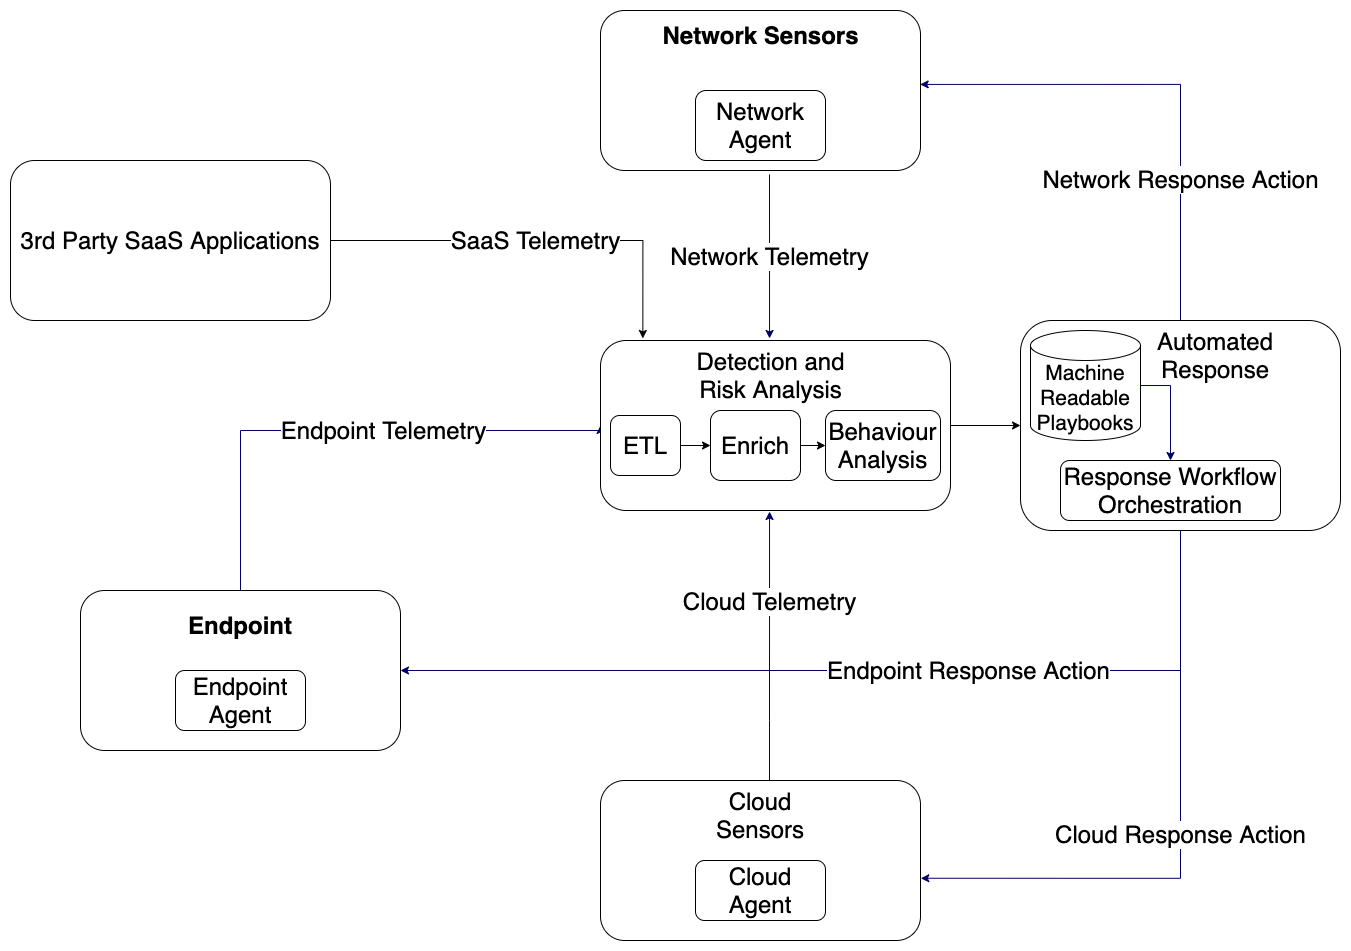
\includegraphics[width=0.8\columnwidth]{usecase/images/security_usecase_analytics_as_a_service_framework.drawio.png}
\centering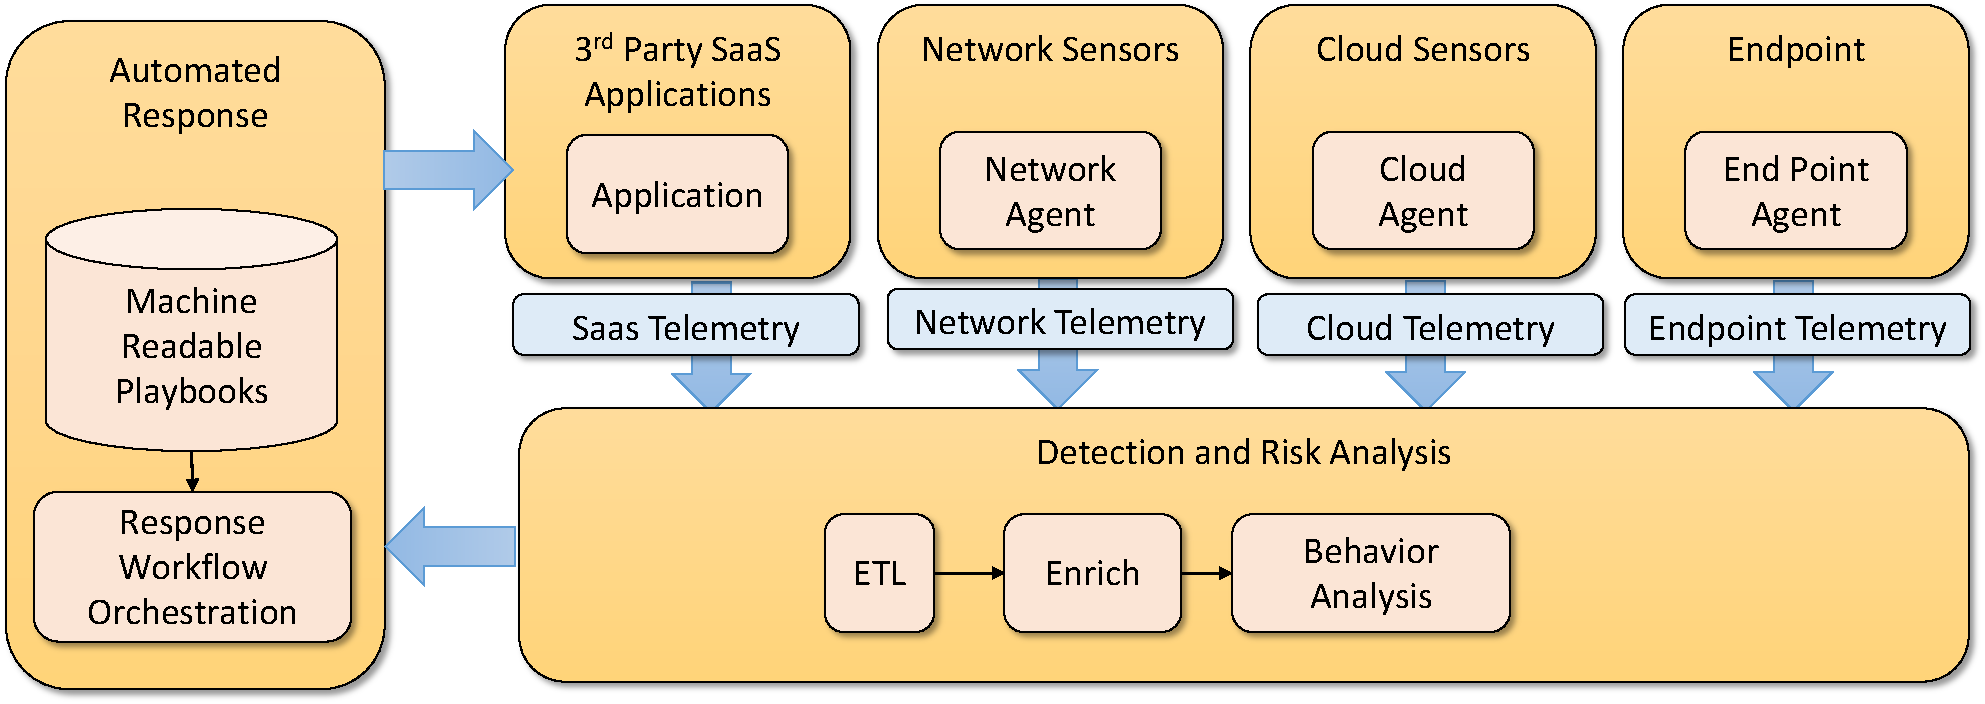
\includegraphics[width=0.8\columnwidth]{usecase/images/nist-security.pdf}

\caption{Continuous Monitoring and Response}
\label{fig:sec-general}
\end{figure}

Figure \ref{fig:sec-general} shows a simplified version of a typical 
Continuous Monitoring Pipeline which usually consists of distributed services for the following functions:

\begin{enumerate}

\item{\bf Telemetry Collection.} Telemetry is typically collected from endpoint, 
network, cloud, and 3$^{rd}$-party Software as a Service (SaaS) applications by endpoint, network, and cloud agents, 
firewalls, Web Application Firewall (WAF), email security, and vulnerability scanners. Telemetry usually consists 
of operating system (OS) and application audit logs, vulnerability scan results, oftware Bill Of Materials (SBOMs), east-west and 
north-south network packets and flow logs, cloud policies etc.

\item{\bf Detection and Risk Analysis.} The Detection and Risk Analysis pipeline 
comprises  extract, transform, and load (ETL) for data normalization, enrichment on normalized data by correlating 
with threat intel from inhouse and 3$^{rd}$ party services, and asset profiling and
behavioural analysis for misbehaviour detection which is done using rule-based 
and machine-learning based approaches.

\item{\bf Automated Response.} Automated Response consists of security response 
playbooks and workflows for alerting, breach containment, mitigation, remediation 
and asset recovery.

\end{enumerate}

This use case has the implicit requirements needing the following
aspects to be addressed by the framework we develop.

\begin{enumerate}

\item{\bf AS vendor neutral cloud and computer service integration.}

  \begin{enumerate}
  
  \item {\bf AS in cloud.} The Analytics Service for this use case is typically hybrid with points of presence on premise where analytics modules can run on the sensors and on cloud. On premise sensors can have support for local storage and running light-weight ETL and machine learning inference, whereas cloud can have more heavy-weight compute and machine learning model training and inference support.
  
  \item {\bf AS in LCCF.} This feature does not apply to the current use case.
  
  \item {\bf AS in microservices.} Microservices approach is highly applicable to the design of continuous monitoring pipeline where each of the subfunctions for telemetry collection, ETL, enrichment, analytics and automated response can consist of several microservices that could either be developed in-house or leverage 3rd party SaaS.
  
  \end{enumerate}

\item{\bf AS architecture.}

  \begin{enumerate}
  
  \item{\bf AS vendor neutral interfaces.} Vendor neutral interfaces would be ideal for different functions of the Continuous Monitoring Pipeline. However, at this time there are no standardized interfaces for technologies related to continuous monitoring. Each vendor typically has its own proprietary set of interfaces and data models and it is upto the consumer of the data to normalize that data.
  
  \item{\bf AS REST.} REST is typically used for human and M2M interfaces at different levels in the Continuous Monitoring pipeline. On-premise and cloud agents for telemetry collection support both data push and pull via REST interface. Data Enrichment services can be in-house and 3rd party SaaS which typically have REST interfaces for pulling reference datasets. Analytics and Automated Response pipelines typically have REST interfaces for pipeline configuration and adding or updating content.
  
  \item{\bf AS layers such as interface, service layer, and provider layer.} Interface layer is required for data access for experimentation and use case development, for configuring and adding new functions and content to telemetry collection, analytics and response functions. Service layer is required to register in-house and 3rd party microservices to support the continuous monitoring pipeline and to register analytics workflows. Provider layer is required to schedule services and workflows on-premise and on cloud.
  \end{enumerate}

\item{\bf AS workflow.}

  \begin{enumerate}
  
  \item{\bf AS catalog and registry.} Continuous Monitoring will comprise several microservices for telemetry collection, ETL, enrichment, analytics, and automated response. These services can be in-house or 3rd party SaaS services running remotely and accessible via APIs. The catalog and registry functionality will be required to catalog and register these services and have required configuration for service setup and service access.
  
  \item{\bf AS cooperation.} There can be intra and inter-function collaboration between the services that are part of the Continuous Monitoring Pipeline. For instance, endpoint, network and cloud agents belong to the telemetry collection function and can have intra-function collaboration where they can cooperate with one another on what telemetry to collect on the fly based on contextual and situational awareness. There is also inter-function collaboration for instance between automated response pipeline and endpoint, network and cloud agents for breach containment, mitigation and asset recovery.
  
  \item{\bf AS competition.} There can also be competing services and rules can be defined on how to orchestrate between these competing services. For instance for instance the Continuous Monitoring Pipeline can have multiple 3rd party and in-house services for threat intel enrichment and rulessets can be defined on how to orchestrate between these services to streamline cost, speed, and resources.
  
  \item{\bf AS orchestrator.} API-based workflow definition, and orchestration capabilities are required for the Continuous Monitoring Pipeline to orchestrate cooperating functions and cooperating and competing microservices that are part of those functions.
  
  \end{enumerate}


\item{\bf AS calculation.}

  \begin{enumerate}
  
  \item{\bf AS with DL.} Deep Learning is leveraged in the analytics stack for behaviour profiling and misbehaviour detection and knowledge graph analysis (e.g., graph neural networks and neuro symbolic analysis).
  
  \item{\bf AS data analytics.} Data analytics is leveraged for data visualization and model quality and drift detection, and visualizing and report generation on security outcomes and alerts. 
  
  \end{enumerate}

\item{\bf AS security.} AS Security is required for securing data at rest and during transit, for securely storing service access credentials, and for enforcing resource access and usage policies. 

\end{enumerate}




% \subsection{Health care}

\TODO{This section does not include how analytics services are used and we use it}

A technician in the hospital uses voice commands to control an MRI
machine to take tomographic images. The images will be automatically
sent to a private analytics service to identify if the images contain
signs of COVID-19. In this case. multiple services are consulted to
assure that the best available and appropriate algorithms are chosen.
Once identified, an image can be sent to a public analytics service
(given patient consent).

\TODO{the following ppg needs more than editing}

In order to improve the available images to improve the deep learning
data analysis. Previous images that have tested negative may be
reanalyzed with the newly improved models. If new cases are found
based on the improved analysis, health care providers are notified,
and further actions regarding the treatment plan by the supervising
physician is cast. As we can see, this example has all the ingredients
that we need to create a new generation of services that integrates
on-premise infrastructure, public and private services. The
orchestration of the services as well as a convenient
interface. Automation of the workflow of this use case example is
explicitly stated.

Analyzing this example, we identify a mixture of services that utilize
on-premise infrastructure (the MRI), private and public services. A
variety of service patterns are used in concert to establish an analysis
pipeline targeted explicitly for this application use case. 

The goal of this work is to analyze the interoperability of such
service scenarios and identify such patterns motivating a vendor
neutral architecture that promotes reusable implementations to 
support aspects of similar use cases addressed by them.




%\FILE{usecase/weather.tex}
\subsection{Use Case: Numeric Weather Prediction}

\paragraph*{Background.} Large amounts of weather data ar e produced continually and stored in
many different databases.  Accurate weather predictions require large
amount s of processing power to accurately simulate conditions
worldwide at a high resolution and fre quent intervals. One of the
most computationally consuming parts of a reliable weather model is th
e microphysics scheme. The current microphysics scheme, Weather
Research and Forecasting (WRF) Single Moment 6-class Microphysics
(WSM6), simulates the processes in the atmosphere that leadto the
formation and precipitation of rain, snow, and graupel and requires
complex floating-point operations needing to be performed on vast
amounts of data for accurate simulations. As computer
performanceimproves, so does the Numerical Weather Prediction (NWP)
models' resolution and accuracy. However, there is still much progress
to be made, as simulation accuracy still falls off sign ificantly for
predictions more than 36 hours in advance. Figure \ref{fig:weather-1}
shows the general WRF modeling system flow chat.

\begin{figure}[htb]
\centering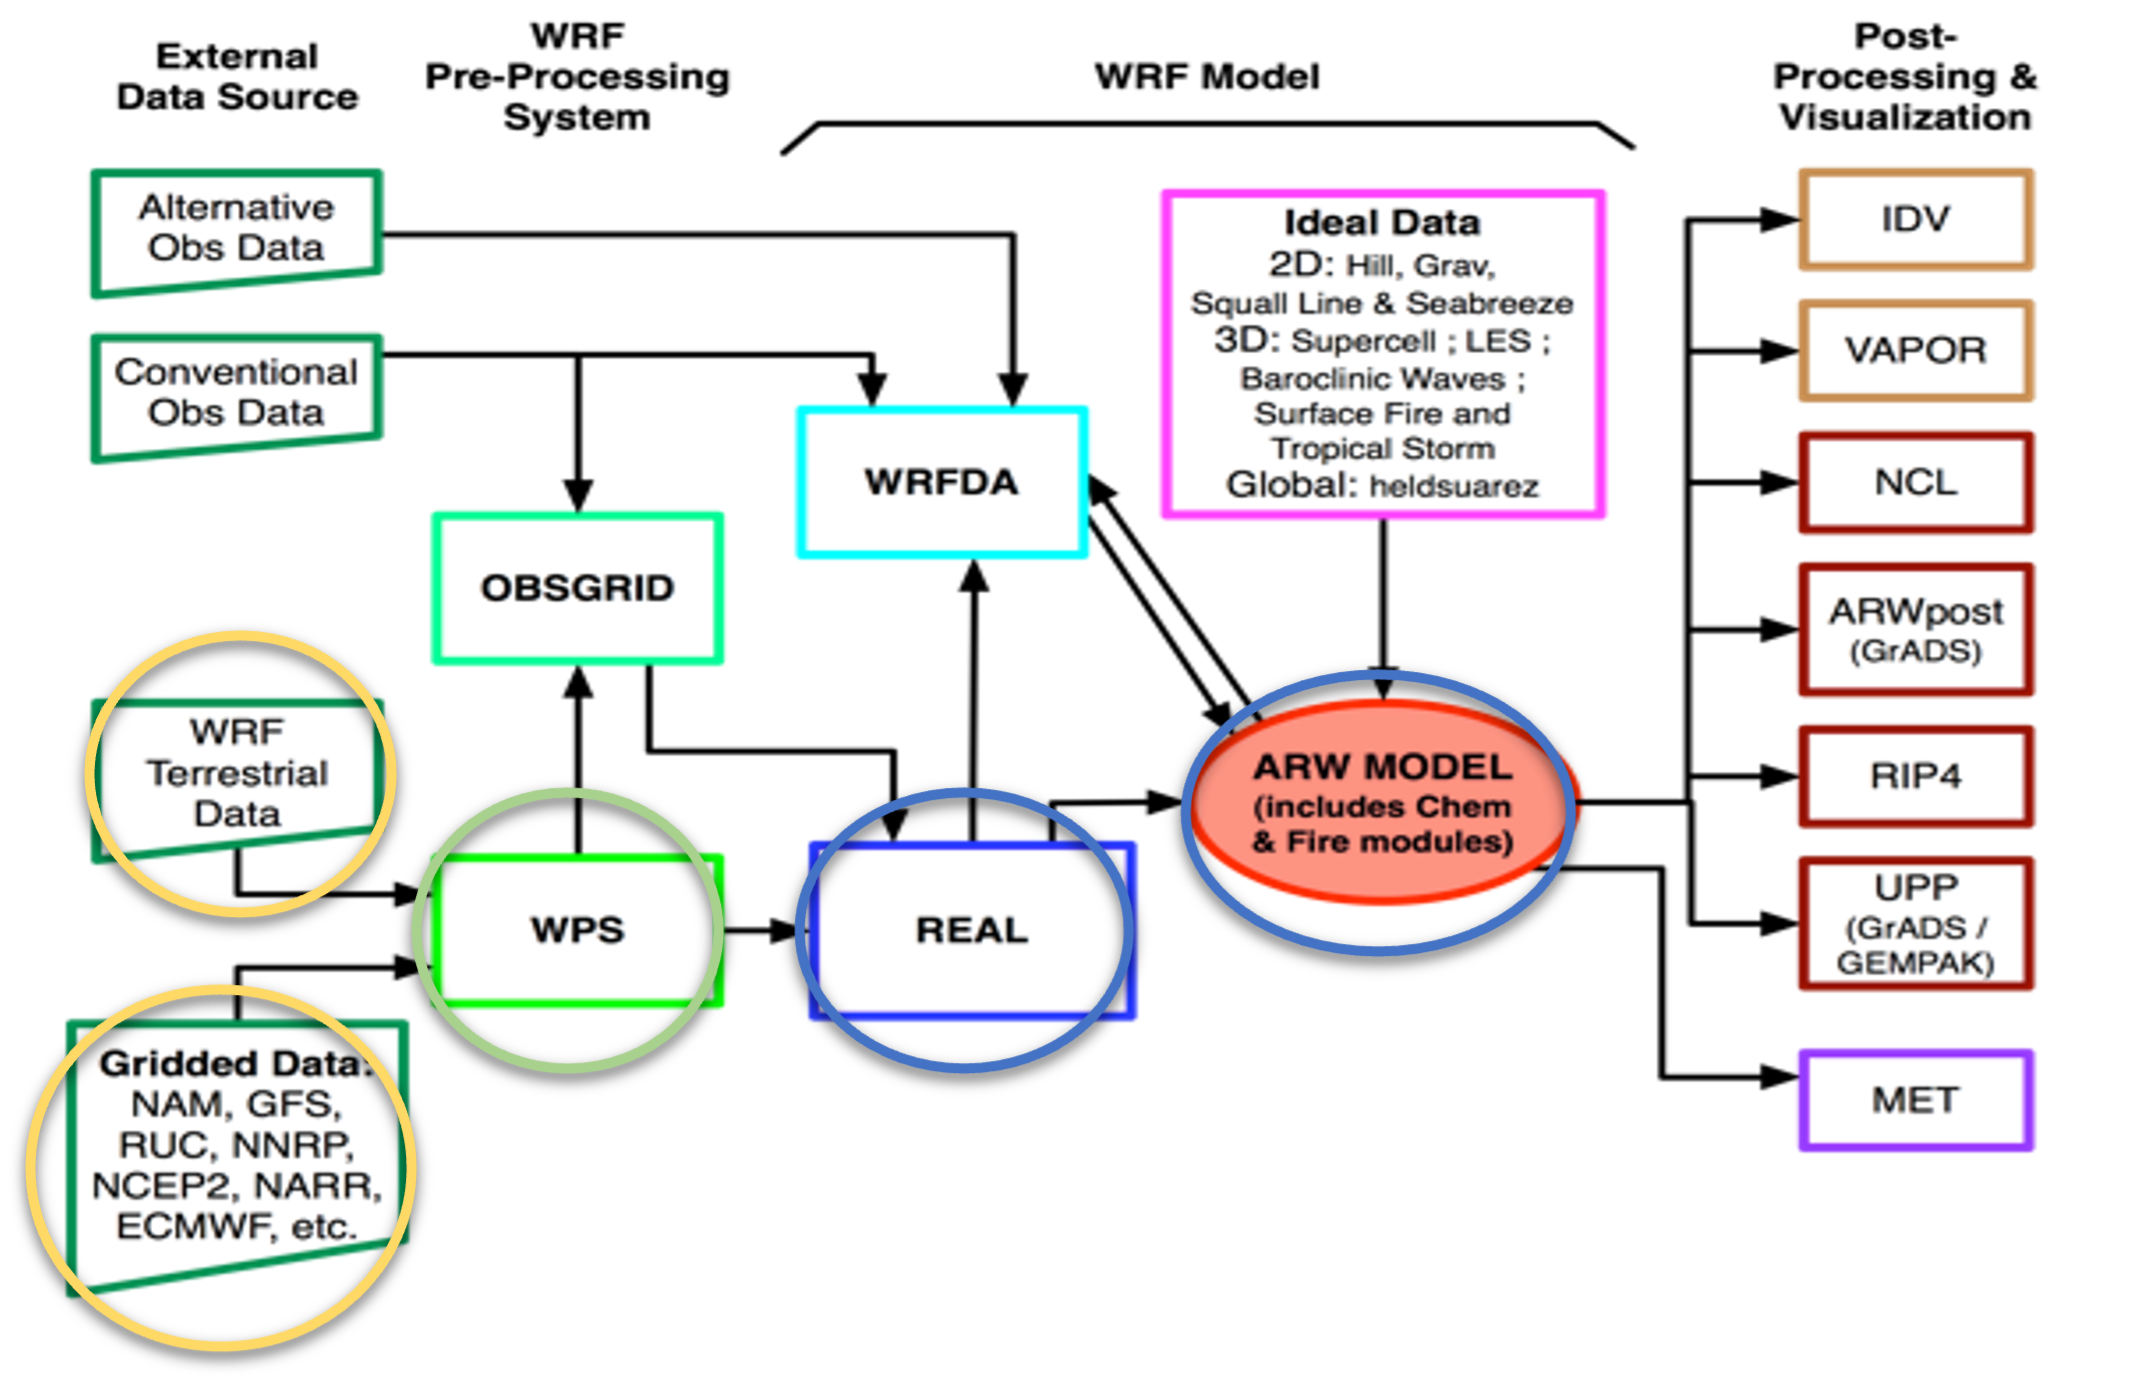
\includegraphics[width=1.0\columnwidth]{usecase/nwp-arch.png}
\label{fig:weather-1}
\caption{WRF Modeling System Flow Chart with Various Configuration.} 
\end{figure}

\paragraph*{Functionalities and Activities} (based on Big Data Application Provider of NBDIF Ref. Architecture).
In this case study, we only focus on two main functionalities, namely
WPS and WRF, and their activities.  Figure \ref{fig:weather-2} shows
the cross-functional diagram for their actions.

WPS Activities:

\begin{figure}[htb]
\centering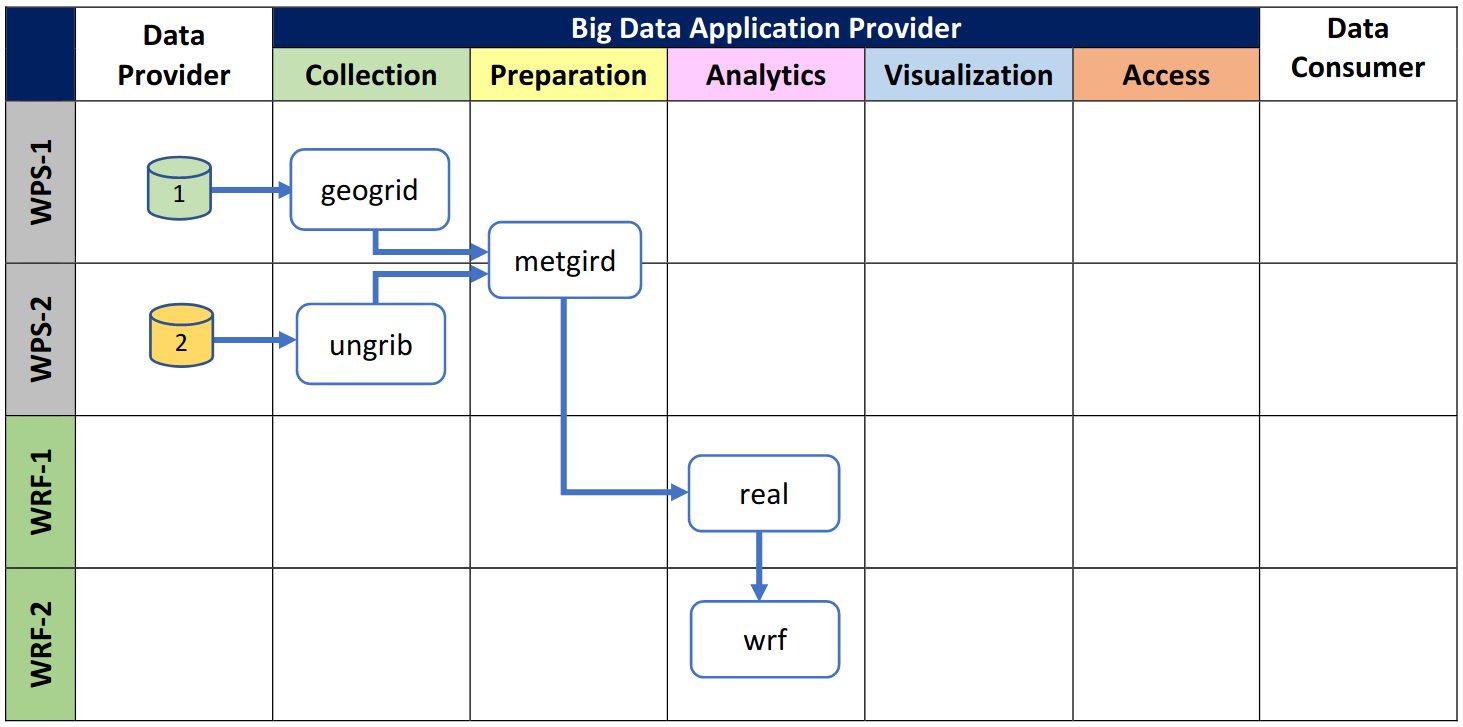
\includegraphics[width=1.0\columnwidth]{usecase/weather.png}
\label{fig:weather-2}
\caption{Cross-Functional Diagram Numerical Weather Prediction.}
\end{figure}

\begin{enumerate}
  
\item geogrid -- defines simulation domains and interpolate various terrestrial data sets to the
model grids. Input data available at [1].

\item ungrib -- extracts needed meteorological data and packs it into an intermediate file format.
Input data available at [2]

\item medgrid -- prepares horizontally interpolate the meteorological data onto the model domain.
  Input data from the output of geogrid and ungrib.

\end{enumerate}

WRF Activities:

\begin{enumerate}

\item real -- prepares vertically interpolates the output from metgrid, and creates a boundary and initial
condition files with some consistency checks.

\item wrf -- generates a model forecast.

\end{enumerate}

\paragraph*{Datasets.}

\begin{enumerate}
  
\item WRF Users Page, WPS V4 Geographical Static Data Downloads Page \cite{wrf-data}

\item NCEP FNL Operational Model Global Tropospheric Analyses, continuing
from July 1999 \cite{cisl_rda_ds083.2}

\end{enumerate}


%\FILE{usecase/hvac.tex}
\subsection{Use Case: HVAC Recommendation}

\TODO{??}{move to authors: Olivera Kotevska, Research Scientist, Oak Ridge National Laboratory, U.S.A.}

\paragraph*{Background.}

Continuous streaming data is produced by heat ventilation and air conditioning (HVAC) systems every
day from the residential houses. This data is stored in a databased on the cloud as it arrives. The data
is used to calculate what should be the next HVAC set point in the house with respect to user
preferences. Periodic recommendations considering environmental parameters, user comfort level
and past user preferences require advanced machine learning algorithm called reinforcement
learning [this sentence needs grammar edit]. Accurate recommendations can save energy and reduce cost. This functionality has three
parts Environmental Forecasting (EF), Learning from the past, (LP), and Set-Point Recommendation
(SPR). EF calculates weather temperature and price predictions. LP learns from the behavior in the
past. SPR model calculates next set-point based on past experience and EF predictions. Figure \ref{fig:hvac-1} shows
the general modeling system flow chat.

\begin{figure}[htb]
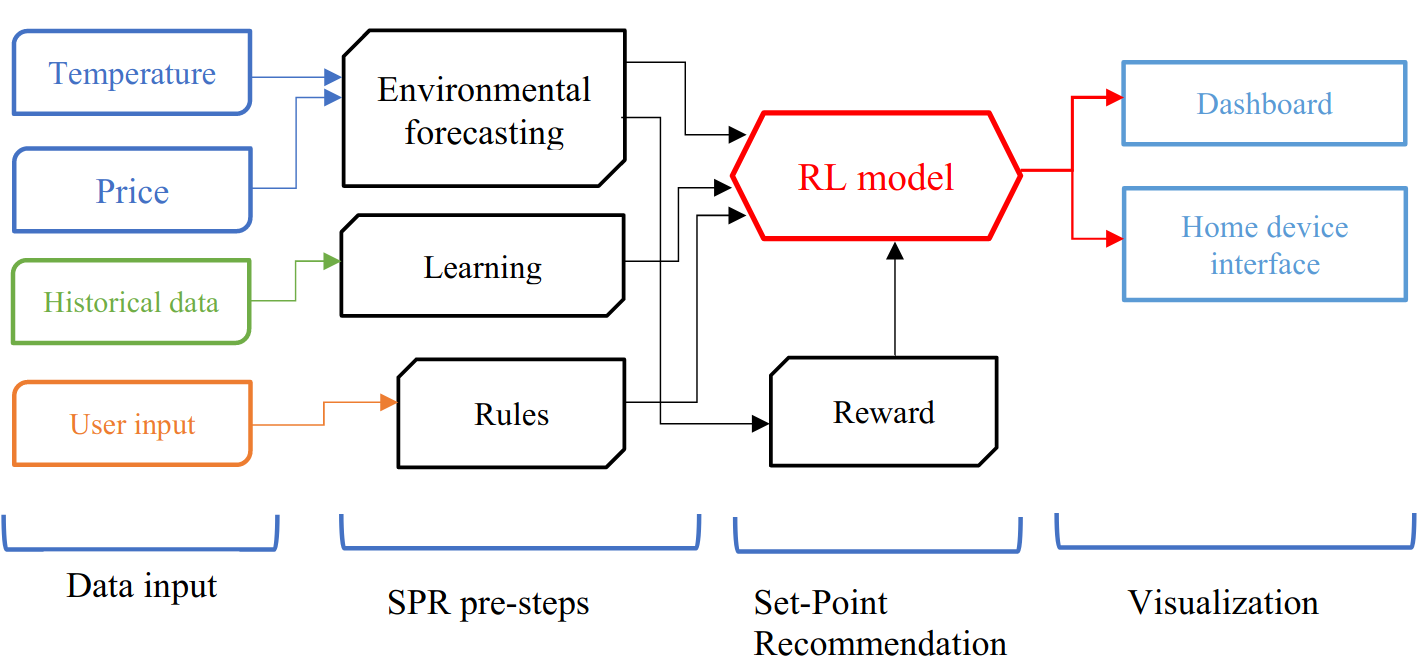
\includegraphics[width=1.0\textwidth]{usecase/hvac.png}
\label{fig:hvac-1}
\caption{HVAC general modeling system flow chat.}
\end{figure}


\paragraph*{Functionalities and Activities} (based on Big Data Application Provider of NBDIF Ref. Architecture).


In this case study, we only focus on three main functionalities, namely EF, LP and SPR, and their
activities. Figure \ref{fig:hvac-2} shows the cross-functional diagram for their actions.



\begin{figure}[htb]
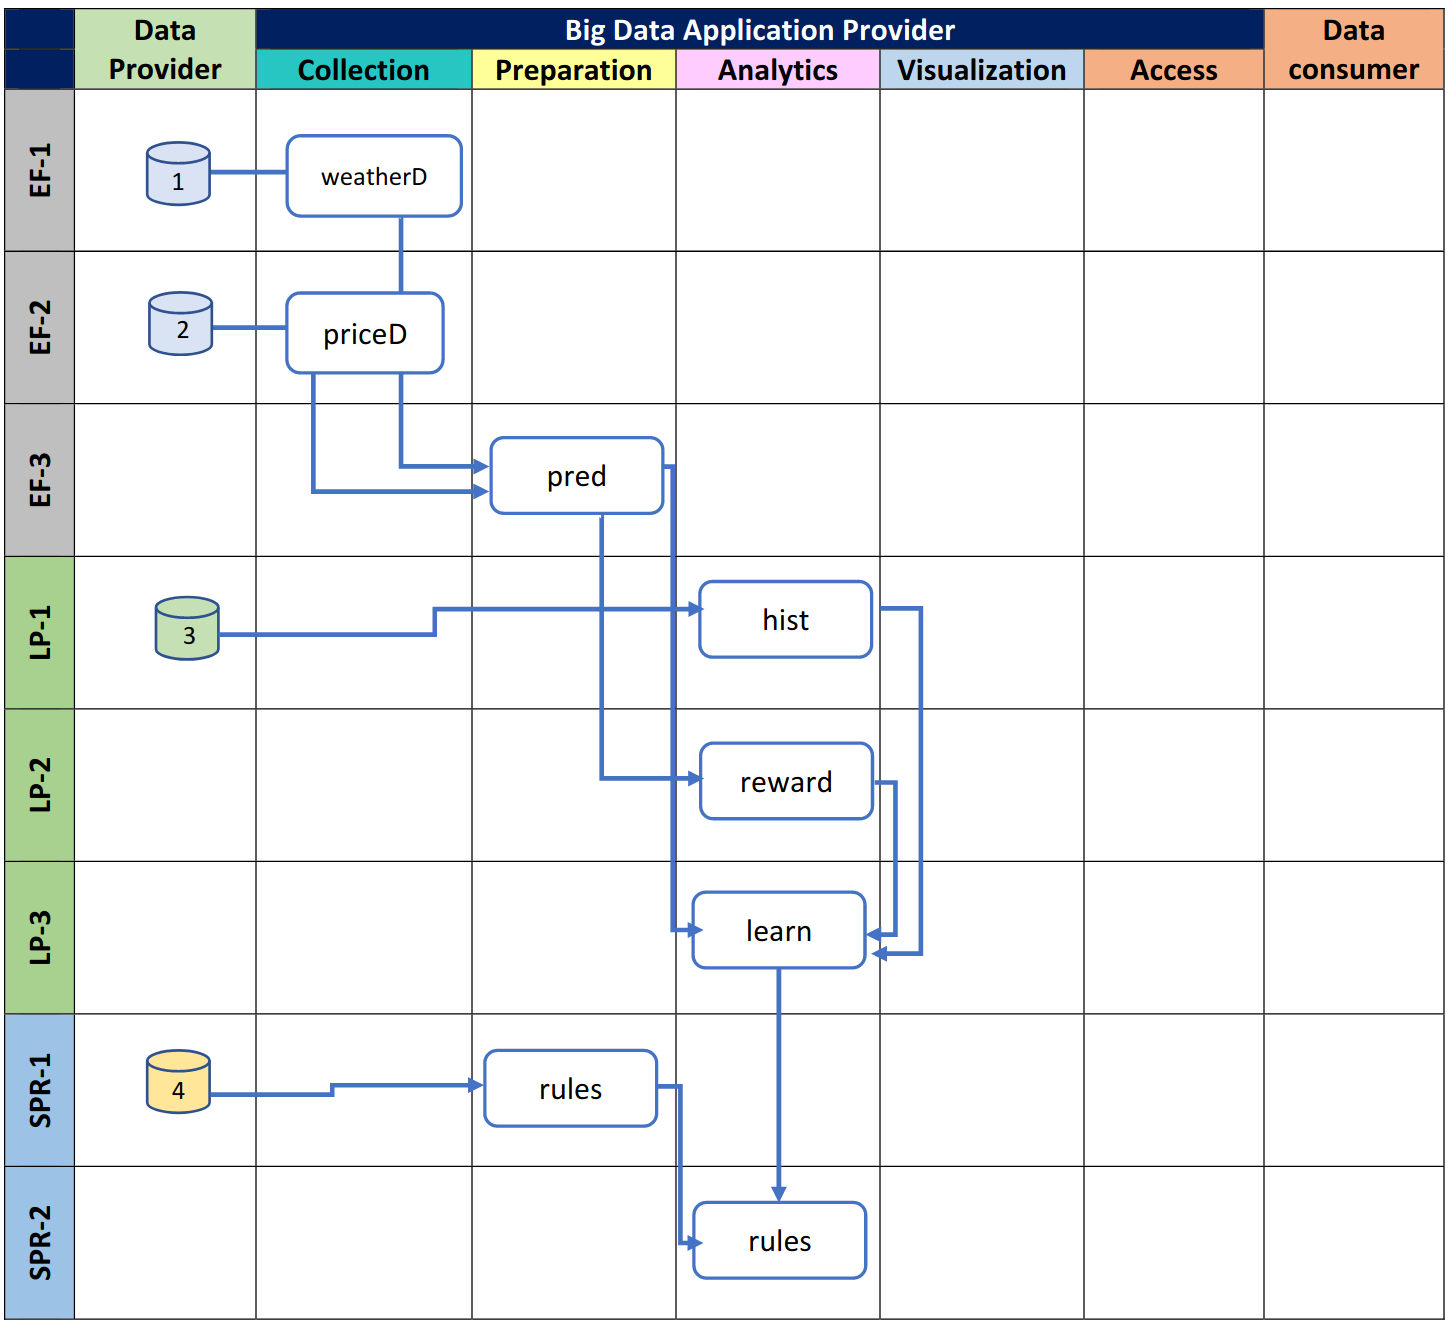
\includegraphics[width=1.0\textwidth]{usecase/hvac-2.png}
\label{fig:hvac-2}
\caption{Cross-Functional Diagram HVAC Recommendation.}
\end{figure}


EF Activities:

\begin{enumerate}
\item weatherD – Collects current weather temperature and predicted temperature for timestamp
X.
\item priceD – Collects current electricity price and predicted price for timestamp X.
\item pred – Extract needed data fields and packs it into an intermediate file format. Input data
from the output of weatherD and priceD.
\end{enumerate}


LP Activities:

\begin{enumerate}
\item hist – Prepares history data points and creates initial condition weights.
\item reward – Generates reward based on the current weatherD and priceD.
\item learn – Collects data from current weatherD, priced, reward.
\end{enumerate}

SPR Activities:

\begin{enumerate}
\item rules – Creates rules based on user preferences and conversion preferences.
\item rlmodel – Interpolates the output from learn, rules and generates set point recommendation
\end{enumerate}

\TODO{??}{No datasets provided.}



\FILE{section-architecture.tex}

\section{Architecture}

TO support the usecases we briefly described and analyzed their requirements, 
we have developed a general architecture that can benefit most analytics services while leveraging and integrating hybrid and multi-cloud  analytics services.

To support our goal to enable the use of hybrid and multi-cloud analytics
services, we are exploring architectural patterns
that are conducive to use cases such as the one we outlined
previously. These patterns are be of general use as they can
be applied to other use cases. In our case, we define an
architecture as depicted in Figure~\ref{fig:arch}.

\begin{figure}[htb]
  \begin{center}
    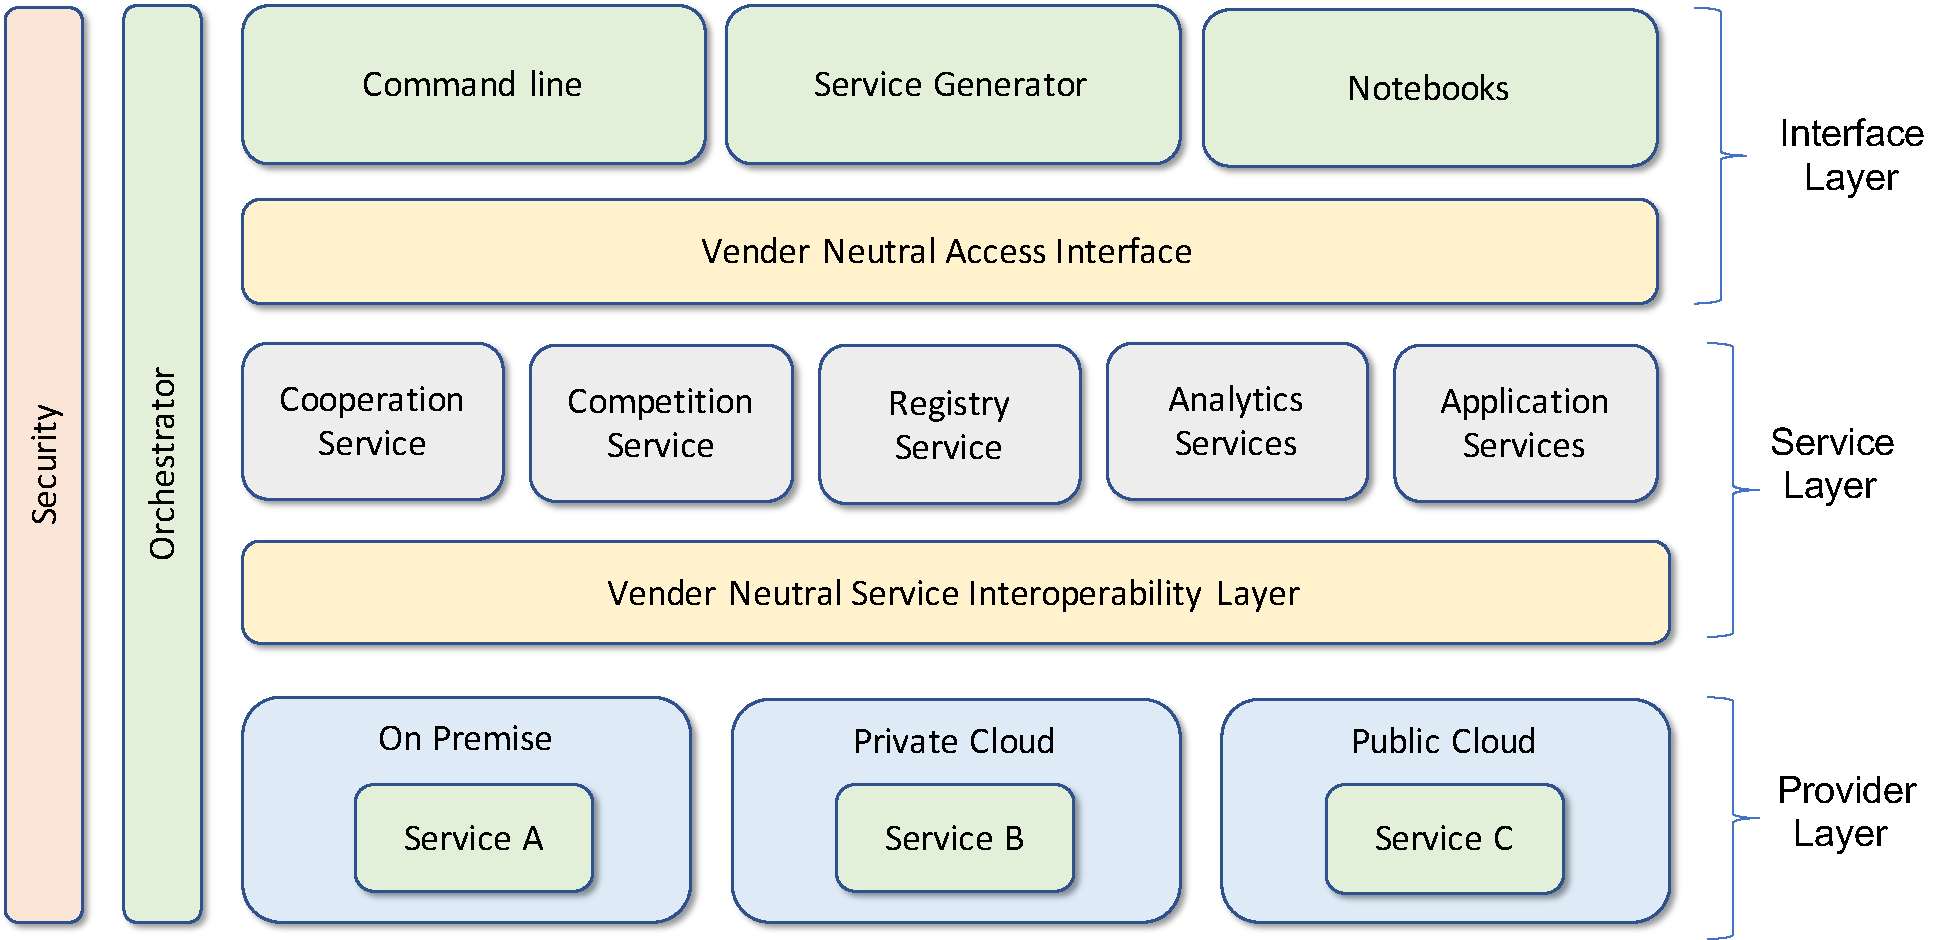
\includegraphics[width=1.0\columnwidth]{images/hybrid-service-arch.pdf}
    \end{center}
  \caption {Architecture of the hybrid multi-analytics service
    framework}
  \label{fig:arch}
\end{figure}

The architecture is organized in layers  and contains
multiple components in each layer. We distinguish the interface,
service, and provider layer. Security and an orchestration service
enable the integration of the various components into a coordinated
application pipeline.

\subsection{Interface Layer}

Today's analytics is invoked through a multitude of interfaces, making
it possible to invoke them in different languages, but also high level
frameworks. This is often achieved by an interface layer using REST
to communicate with the other layers. For our work, we focus on
the command line interface promoting reuse in shells, Jupyter notebooks
showcasing the reuse in an interactive analysis capable framework, and
our previous work to generate REST services (see Section \ref{s:gas}).

\subsubsection{Command Line Interface}

To provide reusability within the DevOps application of data analytics
pipelines, we provide an enhanced command-line interface that
specifically targets hybrid and multi-analytics environments. This is
facilitated by adding command options, shell variables, and
configuration files that can be passed into the commands.
Most importantly, we analyze which specific parameters we
need to make available when investigating cooperative and competitive
services. The parameters can be directly translated to REST service invocations.

\subsubsection{Interactive Notebooks}

Although it is important to provide a command-line interface that can
easily be used to generate computing activities for solving data
analytics tasks, it is even more critical that the framework can be
integrated into interactive steering tasks conducted directly by the
data scientists. For this, we leverage Jupyter notebooks and integrate
service calls to the backend system into the notebooks just as we can
in regular python programs. The difference here is that Jupyter
provides a rich set of interactive components and widgets that can be
leveraged to prototype interactive services but also parameter
studies. While our
previous work has been integrated into notebooks, the capabilities of
notebooks were not yet fully utilized as the integration was done on
the service level but not on a level where Jupyter was used to enhance
the service pipeline. 

\subsection {Service Layer}

\subsubsection{Generalized Analytics Services}
\label{s:gas}

While we have focused previously on the automated generation of
services using REST, we need to consider the other aspects of this
architecture that is needed to support the data analyst. We have
shown that it is possible to create rest services from Python
functions and classes while augmenting them with helper services such
as data uploads. The development of such services is out of the
capability of many data scientists as they focus on developing
transformative data analysis functions and not on the infrastructure
service generation. Our work is lowering the bar for such
implementation and allowing even data analysts to generate reusable
REST services \cite{las21openapi}. The effort to learn how to
create vendor-independent and computer language-independent services
has been reduced from months to days. We can leverage this effort to
generate application-specific services quickly. The services generated
are integrated into a user-managed service registry. We leverage
this service and enabled its exposure via REST through FastAPI as part
of the generator.

\subsubsection{Hybrid Multi-Analytics Service Registry}

\TODO{Gregor: rewrite}

While we have previously developed a simplified generalized service
registry, we are exploring significant extensions to integrate (a)
container images, (b) container services, and (c) analytics 
services offered by service providers. This registry is specially
designed to support cooperating and competing for analytics services.
We intend to add the ability to leverage existing repositories, such as
GitHub and DockerHub to register suitable analytics services as source
code. We will then also add features to provide endpoints to
instantiated services so they can be advertised to a large group of
users. A neutral vendor specification is used as part of the
registry. Such a registry can be hosted by a user or an
organization. We will identify if it is possible to leverage GitHub
for hosting such a registry. This will require a special set of tools
and programs to keep the registry up to date. A user can then
integrate such a registry into their analytics pipeline. New analytics
service specifications can then be either integrated through direct
specifications added to the hosted registry or through the use of
GitHub submodules. Using submodules offers the ability to keep up to
date with analytics services developed by others and allows updates
through automated DevOps-controlled pull requests. This registry
technology would completely replace our earlier registry work if
successful. It would also allow the integration of private services as
private analytics services can be integrated while using private
submodules hosted in private repositories. Hence, the details of such
modules are not exposed. As GitHub also supports GraphQL we will
explore using GraphQL as a mechanism for the specification of Registry
entries. To increase privacy, git can also be hosted on-premise.

\subsection{Application Services}

An application may require the availability of very specific
application-oriented analytics services. Our architecture allows us to
integrate them while reusing the same vendor-neutral specification
format. This includes not only cloud services but also the
integration of analytics services that rely on on-premise
infrastructure. An example would be access to a supercomputer in the
TOP500 list that is used to conduct a complex data analytics task
reusing GPUs to conduct deep learning for COVID-19 analysis. This
results in two specifications. A general specification that can be
reused on other similar on-premise computers, and a second that is
specifically targeted to the targeted on-premise infrastructure. This
could include the integration of hosted data services or specific
network capabilities.

\subsection{Analytics Services}

Data analysts are developing analytics functions on a regular
basis. As we can use our service generator to transform them into
analytics services, we will be able to create and register them into
our registry. We will expand upon our available services but focus on
services that explicitly address multi-cloud and hybrid service use
cases.

A good example may be natural language processing to analyze a text
with either a local service, a loud hosted service by different
vendors. Here, based on input parameters, we create an overarching
language analytics service that chooses the various services with the
the help of service level requirements and agreements.

\subsection{Cooperation and Competition Services}

As previously indicated, we already have identified two special use
cases of data analytics services that leverage hybrid and
multi-analytics 
services. This is the specification of services that
employ:


\paragraph{Cooperation.} Cooperating services are services that use one or
more services from hybrid multi-analytics services. They are
cooperating together to address the solution to a formidable data
analytics problem. Thus the resources form a "team" of services that
work together. This includes the integration of specialized services
that may not be unique to a particular provider. Still, it also could
mean that computational analytics processes could be performed in
parallel, and results could be gathered to accelerate the analytics
task. A parameter study is a very good example of one kind of
cooperating services

\paragraph{Competition.} Here, the available hybrid multi-analytics services
directly compete with each other. This can be done by direct selection
of services that are more suitable than others. This selection could
be based on resource requirements such as time, availability, cost,
and feature. However, the framework could take "observations" and
propose automated conclusions about which services to choose from. A
possibility would even be to integrate deep-learning strategies into
the selection process.
  

\subsection{Provider Layer}

An integral part of the proposal is identifying how we can leverage
services from multiple providers, including on-premise services. We
have shown in our previous work that we can specify vendor-neutral
specifications to access, for example, virtual machines. We will expand
this concept while using the concept of containers. However, we also
need to identify services that are offered by
multiple vendors, such as language processing services. Although they
can be directly accessed via vendor-specific interfaces. It will
be important to identify if they can be generalized so the users
can benefit from a uniform vendor-neutral service interoperability
layer. We will identify a usability example to explore the
possibilities of this approach.

\subsection{Crosscutting Services}

We have two crosscutting services. One is the {\em orchestrator} that
allows the specification of service pipelines to combine the various
services that are needed for application implementation. The other
is a {\em security} service that will enable us to access the various services
through the required authentication and authorization mechanisms. The
latter we have demonstrated in {\em cloudmesh} where users can manage their
own access to a multi-cloud environment ta access their activated
analytics services. We will leverage from that effort but  also leverage from
open source solutions that can be embedded in our vendor-neutral
service specification, such as basic and OAUTH security. In general, we
abstract the security calls to be callouts to the appropriate
authentication mechanisms.



\FILE{section-defining.tex}

\section{Defining and Finding Reusable Analytics Services}
\label{sec:defining}

\TODO{Defining and Finding Reusable Analytics Services is an importeant aspect of usability of services. We will include
the definition and conceptual architecture of reusable analytics services. This includes the
following concerns that are organized as subsections.}


\FILE{section-fair.tex}

\subsection{AS-FAIR-DO: Analytics Service FAIR Principle}
\label{sec:fair}

To project easy reusability, we strive towards the implementation of
the AS-FAIR-DO principle for analytics services. The FAIR principle is
typically applied to data and as such we can apply it the metadata
associated with analytics services. The FAIR principal addresses who
to be findable, be accessible, be interoperable, and be reusable. In
Figure \ref{fig:as-fair-do} we explicitly augmented the general FAIR
principle with terminology so it can apply to analytics services. The
augmentations are colored in red.

\begin{figure}[htb]
\centering\resizebox{1.0\columnwidth}{!}{
\begin{tabular}{p{1cm}p{8cm}}
\multicolumn{2}{l}{To be Findable:} \\
F1 & \textcolor{red}{analytics services metadata} are assigned a globally unique and persistent identifier \\ 
F2 & \textcolor{red}{analytics services} data are described with rich metadata (defined by R1) \\
F3 &  \textcolor{red}{analytics services metadata} clearly and explicitly include the identifier of the data related to the analytics services it describes \\ 
F4 & \textcolor{red}{analytics services metadata} are registered or indexed in a searchable resource \\
\multicolumn{2}{l}{To be Accessible:} \\
A.1 &  \textcolor{red}{analytics services metadata} are retrievable by their identifier using a standardized communications protocol \\
    A1.1 & \textcolor{red}{analytics services} the protocol is open, free, and universally implementable \\
    A1.2 & the \textcolor{red}{analytics services} protocol allows for an authentication and authorization procedure, where necessary \\ 
A.2 & \textcolor{red}{metadata} are accessible, even when the data are no longer available \\
\multicolumn{2}{l}{To be Interoperable:}\\
I1. & \textcolor{red}{analytics services metadata} use a formal, accessible, shared, and broadly applicable language for knowledge representation. \\
I2. &  \textcolor{red}{analytics services metadata} use vocabularies that follow FAIR principles \\
I3. &  \textcolor{red}{analytics services metadata} include qualified references to other metadata \\
\multicolumn{2}{l}{To be Reusable:} \\
R1. & \textcolor{red}{analytics services metadata} are richly described with a plurality of accurate and relevant attributes \\
R1.1 & (meta)data are released with a clear and accessible data usage license \\
R1.2 & (meta)data are associated with detailed provenance \\
R1.3 & (meta)data meet domain-relevant community standards \\
\multicolumn{2}{l}{To be Deployable:}\\
D.1 & \textcolor{red}{analytics services metadata describing deployability aspects} \\
\multicolumn{2}{l}{To be Operational:} \\ 
O.1 & \textcolor{red}{analytics services metadata describing operational aspects} \\ 
\end{tabular}
}
\caption{Fair guiding principles adapted to analytics services:
  Analytics Services - FAIR - Deployable and Operational
  (AS-FAIR-DO).}\label{fig:as-fair-do}
\end{figure}



\FILE{section-catalog.tex}

\subsection{Analytics Service Catalogue}
\label{sec:catalog}

\paragraph*{Motivation.}
Cloud providers offered a considerable set of analytics services to
their customers. There are many analytics services available. A user
needs to be able to quickly obtain an overview of such available
services. This helps identifying further actions in order to evaluate
them and identify if further investigation is justified. The catalouge
contains enough details to locate the service and evaluate if it is
useful. However, it may not provide technical details which are
captured by a service registry instead.

\paragraph*{Access Requirements.}
The catalogue may be public or may be restricted while authorized
entities may access it. As analytics services may evolve over time,
time dependent versioned descriptions of the services must be able to
be included. An organizational entity may manage their own
catalogues. It is desirable to have the catalogues be uniform, so that
they can be combined into a larger catalogue combining entries of
multiple organizations.

\TODO{8.2.4.2 and 8.2.4.4 and 8.2.6.2 are all labelled Access
  Requirements. perhaps we should be more specific}

\paragraph*{Federation.}
The offerings are typically limited to a particular vendor. Users can
benefit from a federates service catalogue to search and explore for
needed services by the user. In contrast to a registry a catalogue may
not include all technical details but could in contrast include
services that lack such details and thus can be the basis of an
exploratory process.  A Federated analytics service repository is
planned to be hosted on GitHub (LINK TBD) The catalogue contains the
following attributes, many of which are also used in an analytics
service registry.

The catalogue is organized as a list of entries, where each entry
contains a number of attributes. These attributes may be required or
optional. We list in Table \ref{tab:cat}.


\begin{table}[htb]
\caption{Catalouge attributes}
\label{tab:cat}
\resizebox{1.0\columnwidth}{!}{%
\begin{tabular}{p{3cm}p{6cm}p{0.2cm}}
Name	& Description	& \rotatebox{90}{Required} \\
\hline
ID	& UUID, globally unique	& \OK \\
Name	& Name of the service	& \OK \\
Title	& Human readable title 	& \OK \\
Public	& True if Public 
(needs use case to delineate what pub private means) & 	\OK \\
Description	& Human readable short Description of the Service	& \OK \\ 
Version	& The version number or tag of the service	& \OK \\
License	& The license description	& \OK \\
Microservice & 	\OK/No/Mixed	& \OK \\
Protocol	& REST	& \OK \\
Owner	& Name of the distributing entity, organization or individual. It could be a vendor.	& \OK \\
Modified	& Modification Timestamp (when first same as created)	\OK \\
Created	& Date on which the entry was first created	& \OK \\
Documentation	& Link to a URL with detailed description of the service	& \OP \\
Source	& Link to the source code if available	& \OP \\
Tag(s)	& Human readable common tags that are used to identify the service that are associated with the service	& \OP \\
Category(s)	& A category that this service belongs to (NLB, Finance, ...)	& \OP \\ 
Specification/ Schema	& Pointer to where schema is located &	\OP \\
Additional metadata	& Pointer to where additional is located including the one here.	& \OP \\
Endpoint	& The endpoint of the service	& \OP \\
SLA/Cost	&	& \OP \\
Authors	& contact details of the people or organization responsible for the service (freeform string)	& \OP \\
Data	& Description on how data is managed	& \OP \\
\hline
& \OK = required; \OP = optional, \NA = not applicable
\end{tabular}

}

\end{table}



\FILE{section-registry.tex}

\subsubsection{Analytics Service Registry}
\label{sec:registry}

\paragraph*{Motivation.} 

The goal of a federated analytics service registry is to establish
federated registries to locate and consume analytics services with
persistent identifiers across organizations.

A service registry can serve as a public, private, or federated
registry. The first two properties define whether the registry is public or
private. In the case of a private registry, proper security measures need
to be taken into account to govern access. Our framework does not make
any recommendations about the security framework chosen and it is up
to the implementer to specify it. In the case of a federated registry,
more than one registry can be joined, to provide the user the
impression of a single registry.

Within the analytics services, we distinguish two classes. The first
class are instantiated (running) services that are offered by a
service provider and allow direct reuse. The second class are library
providers that distribute analytics activity not as an instantiated
service, but as a source code library which can be deployed as a
service.


A simple use case can be formulated as follows.
A user wants to find an analytics service and needs to
identify candidate services based on their descriptions and
features. A user wants to find services quickly and therefore expects
modern keyword search and taxonomy, faceted search, query
functionalities; as well as descriptions that facilitate location and
identification of relevant and appropriate analytics services, from the
registry.

The registry contains enough details to not only locate the service,
but also how to use it.

\paragraph*{Access Requirements.} 

% \TODO{possibly change section to privacy requirements so that LoA
% and Authentication can be moved to a separate section ?}

Public Analytics Service Registry. Public analytics discovery
services are intended to allow users to find publicly hosted
services. The information provided includes the provider, [x], and
[y], and / thus reduces users' efforts in locating relevant services.

\begin{description}

\item[Levels of Assurance (LoA) in User Identity.] Most readers should
  be familiar with functionality to {\em sign in with ORCHID, or
    Facebook} or something known to the user. In general identity
  management scenarios, this provision enables what is referred to as
  {\em guest identities}, which is useful for many users who are
  interested in invoking low-level activities or less sensitive
  operations. With respect to federated service authentication and
  authorization, OIDC guest identities meet a low level of
  assurance. In contrast, users with higher LoAs are afforded
  permissions to perform to privileged activities or gain access to
  more sensitive xyz.

\item[Multi factor Authentication in User Identity.] A means for
  authenticating users via two or more types of
  authentication. An MFA instrument can elevate a user's level of
  assurance profile. RAF and IGTF are examples of such assurance
  framework standards.  OpenID Connect, SAML, and X.509 are examples
  of services that expose interfaces for multiple authentication.

\item[Private Analytics Service Registry.] Analytics Services stored
  in private registries are only available to authenticated and
  authorized / member users. Private registries allow providers to
  build virtual organizations [/ VOMS] that advertise specialized
  services to its user community. In contrast to a public analytics
  registry, access controls in private registries are more
  restricted. In addition, different group privileges may restrict the
  visible analytics service to the user (see related sections on
  user identity and levels of user privilege).

\item[Federated Analytics Service Registry.] A user wants to make
  selection decisions regarding which service to use. Analytics
  service brokers and providers therefore offer a federated analytics
  service in which multiple services from multiple providers are
  included. Rather than having to visit multiple, separate providers'
  registries, the user can visit the federated registry of the
  analytics broker to look up all potentially suitable services, via a
  single interface and browser. It may be expected that federated
  registries abstract the technical effort that casual users would
  experience during location and inspection of published analytics
  services.  Underlying analytics service registry technologies
  leverage cross-organization persistent identifiers, enhanced with
  information that the original service provider may not have
  available, and xyz. such "enrichment" may could include, for example,
  cost comparisons, or (some type of) ratings from its user community.

\item[Enhanced Analytics Service Registry.] Both public and private
  registries may need to be enhanced by providing detailed information
  so the user has a better understanding of the offering and allows
  comparison to similar artifacts maintained and published in the
  registry. Information details may include, for example, benchmark
  information, service level agreements, or cost measures such as
  carbon cost, or technical limitations such as storage access and
  availability for big data.
  
\end{description}

\paragraph*{Registry Namespace.}
To allow uniform integration of entries into a unified namespace, URLs
are used to distinguish the services. This includes two different
entities. Firstly, an entity that defines the code base of a
service. Such a code base could be for example hosted on publicly
accessible code repositories. Secondly, the namespace could include
instantiated analytics service endpoints that define a running
instance of an analytics service.

The attributes are listed in Table \ref{tab:reg}. Some attributes may
be optional and may be dependent on whether they are deployed services, or
contain a library that may be deployed.


\begin{table}[htb]
\caption{AS services Catalog and Registry attributes}\label{tab:reg}
\resizebox{1.0\columnwidth}{!}{%
\begin{tabular}{|p{3cm}|p{5cm}|p{0.25cm}|p{0.25cm}p{0.25cm}|}
\hline
&             & \rotatebox{90}{Catalog provider} & \rotatebox{90}{Service provider} & \rotatebox{90}{Library provider} \\
Name & Description & & \multicolumn{2}{l}{Register} \\
\hline
ID & 	UUID, globally unique &	\OK & \OK &	\OK \\
Name & 	Name of the service	& \OK & \OK	& \OK \\ 
Title & 	Human readable title & \OK &	\OK	& \OK \\
Public	& True if Public
(needs use case to delineate what pub private means) &  \OK &	\OK & \OK \\
Description	& Human readable short Description of the Service	& \OK & \OK & 	\OK \\
Endpoint &	The endpoint of the service	& \OK & \OK	&  \NA \\
List of Input Parameters &
	A list of parameters to the service. The parameters have each the form of name, function, type, value, and access. The type indicates the data type. The access indicates if the parameter is a data stream, database, single value/function, or event.
The function responds to a different function in case multiple are provided by the service.	& \OP & \OK	& \OK \\ 
List of Output Parameters 
  style (event, stream, data)
  value
  timestamp & 
	List of responses cast by the service. The responses have the form of function, name, type, value, access, and timestamp. The type indicates the data type. The access indicates if the parameter is a data stream, database, single value/function, or event.
The function responds to a different function in case multiple are provided by the service. &  \OP &  	\OK  & \OK \\
Version	& The version number or tag of the service	& \OK & \OK	& \OK \\
License	& The license description	& \OK & \OK	& \OK \\
Protocol & 	Example: REST	& \OK & \OK	& \OK \\
Microservice & 	True if microservices used & \OK & \OK	& \OK \\
Modified & 	Modification Timestamp	& \OK & \OK& \OK \\
Owner	& Name of the distributing entity, organization or individual. It could be a vendor.	& \OK & \OK	& \OP \\
Author &	Contact details of the people or organization responsible for the service	& \OK & \OP	& \OK \\
Tags &	Human readable common tags that are used to identify the service that are associated with the service	& \OK & \OP & \OP \\
Categories &	A category that this service belongs to (NLB, Finance, ...)	& \OK & \OP & \OP \\
Created	& date and time on which the analytics service was instantiated or created	instantiated	& \OK & \OK & \OK \\
Heartbeat &	State and timestamp of the last check when the service was active	& \NA & \OP & 	\NA \\
Documentation &	Link to a URL with a detailed description of the service
Source	Link to the source code if available	& \OK & \OP & \OP \\
Specification/Schema &	Pointer to where specification schema is located	& o & \OK &  \OK \\
AdditionalMetadata	& Pointer to where additional is located including the one here.	& \OP & \OP &	\OP \\
SLA	& Serves level agreement including cost	& \OP & \OP 	& \OP \\
CachingInterval	&If a service is accessed a lot, the caching interval can be used to put a limitation on the Response with an LRU cache	& ? & \OP &	\NA \\
DataIntegration &	In case of big data the data cannot be provided as a parameter to the analysis function. Instead, we need to provide the data as endpoint. However, often tata may need to be uploaded or can be downloaded. In this case this field provides the upload and download endpoints and the protocol to access the data	& \OP & \OP &	\OP \\
Authors	& contact details of the people or organization responsible for the service (freeform string)	& \OK & \OK & \OK \\
\hline 
\multicolumn{5}{l}{\OK = required; \OP = optional, \NA = not applicable}\\
\end{tabular}
}

\end{table}

\paragraph*{Benefits of a federated analytics service registry}

A service registry can publicize and improve end-user access to data
from different sources, by overcoming some of the challenges inherent
in describing and surfacing document content and format. Publication,
and discovery of information resources are enriched with metadata
enabling the findability and reusability of a service supporting the
FAIR principle. While describing the interfaces and allowing for the
instantiation or the reuse of already instantiated services we address
the accessibility and interoperability. With respect to analytics as a
service, end users should be able to find various analytic services
and similar services without having to individually search multiple
locations or databases, each built to operate on its own, unique
storage and retrieval constructs. Through these descriptions automated
service integration can be provisioned while targeting not only the
functionality involved, but also allowing service level considerations
to be addressed. Furthermore, such analytics services could provide
significant security implications such as the protection of a database
while only exposing a subset of approved analytics functions that are
executed on the data sets. This includes partial and controlled
sharing of data mashups that can be made available to the community and
registered to make reuse easier without everyone having to replicate
the service.



\FILE{section-federation.tex}

\section{Service Federation}
\label{sec:federation}


This section discusses aspect of federated registries to locate and
consume analytics services with persistent identifiers across
organizations.


This is not the term is at this time in the document not properly used.

We use so far 

(1) federation of catalog and registry

(2) federation of services stored in the registry and catalog

(3) federaion of services through high level services delegatiing to other services. 

We will clarify this and appropriately address.


\FILE{section-workflow.tex}

\subsubsection{Analytics Service Pipelines}

\paragraph{Motivation.}
In many cases a big data analysis is split up in multiple
subtasks. These subtasks may be reusable in other analytics
pipelines. Hence it is desirable to be able to specify and use them in
a coordinated fashion allowing reuse of the logic represented by the
analysis. Users must have a clear understanding on what the analysis
is doing and how it can be invoked and integrated.

\paragraph{Access Requirements.}
The analysis must include a clear and easy to understand specification
that encourages reuse and provides sufficient details about its
functionality, data dependency and performance. Analytics services may
have authentication, autorotation and access controls build in that
enable access buy users controlled by the service providers.



\begin{figure}[htb]
\centering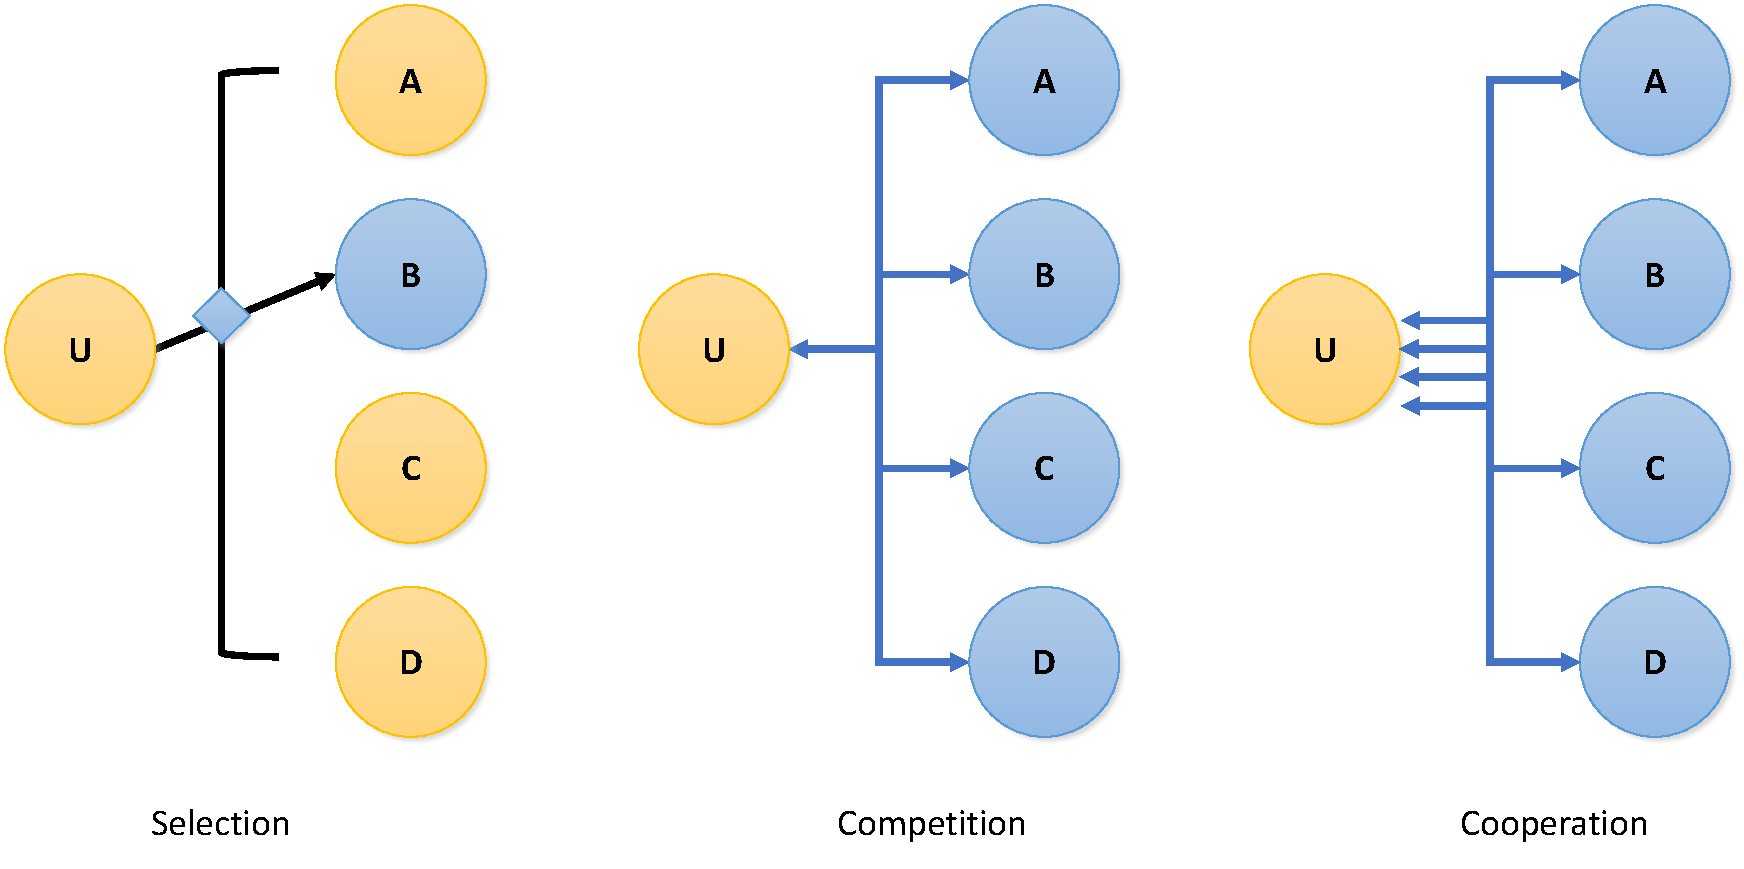
\includegraphics[width=1.0\columnwidth]{images/NIST-AI-services-workflow.pdf}
\label{fig:hvac-2}
\caption{Hybrid service integration.}
\end{figure}


\subsubsection{Workflow Controlled Computing}

High-performance computing (HPC) is for decades a very important tool for science. Scientific tasks can leverage the processing power of a supercomputer so they can run at previously unobtainable high speeds or utilize specialized hardware for acceleration that otherwise are not available to the user. HPC can be used for analytic programs that leverage machine learning applied to large data sets to, for example, predict future values or to model current states. For such high-complexity projects, 
there are often multiple complex programs that may be running repeatedly in either competition or cooperation. This may include resources in the same or different data centers. We developed 
a hybrid multi-cloud analytics service framework that was created to manage heterogeneous and remote workflows, queues, and jobs. It can be used through a Python API, the command line, and a REST service. It is supported on multiple operating systems like macOS, Linux, and Windows 10 and 11. 
The workflow is specified via an easy-to-define YAML file.
Specifically, we have developed a library called Cloudmesh Controlled Computing (cloudmesh-cc) that adds workflow features to control the execution of jobs on remote compute resources, while at the same time leveraging capabilities provided by the local compute environments to directly interface with graphical visualizations better suited for the desktop. The goal is to provide numerous workflows that in cooperation enhances the experience of the analytics tasks. This includes a REST service and command line tools to interact with it.


\begin{figure}[htb]
\centering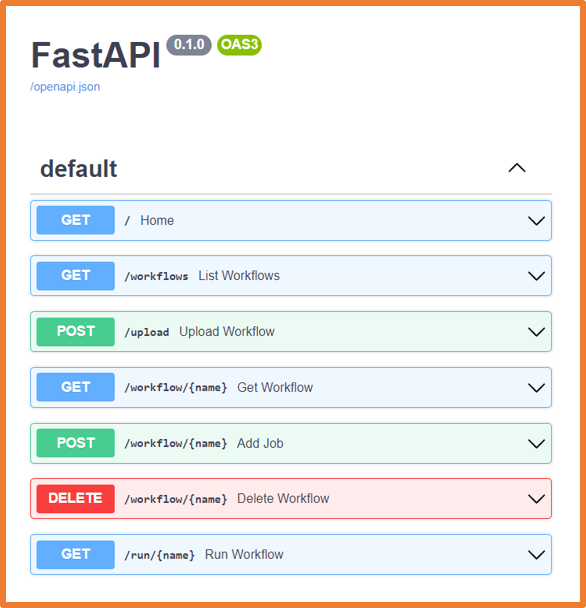
\includegraphics[width=0.7\columnwidth]{images/fastapi-service.png}
\caption{Fast API Workflow Service.}
\label{fig:fastapi-cc-arch}
\end{figure}

\begin{figure}[htb]
    \centering
    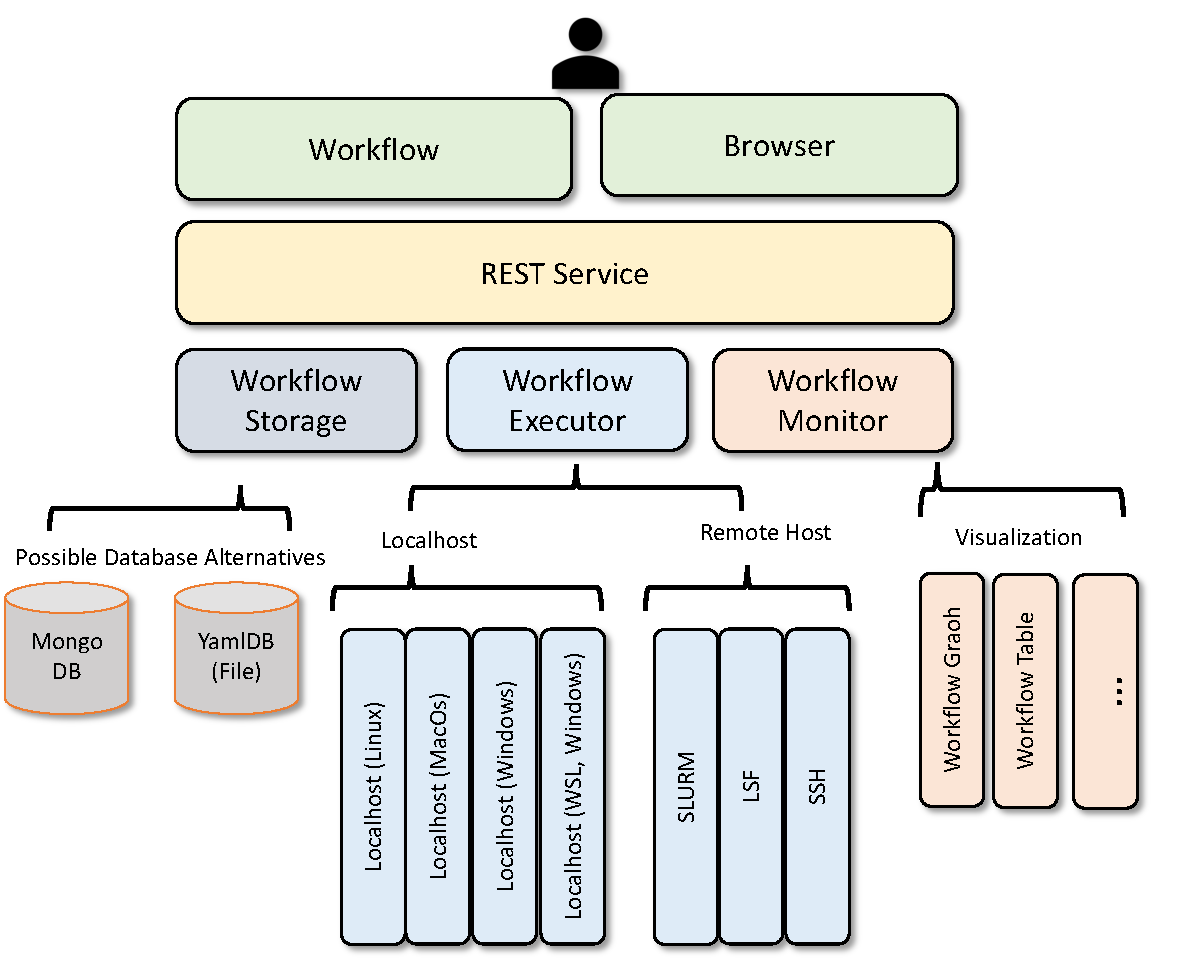
\includegraphics[width=1.0\columnwidth]{images/cc.pdf}
    \caption{Architecture Workflow Service.}\label{fig:cc-2}
\end{figure}

\begin{figure}[htb]
    \centering
    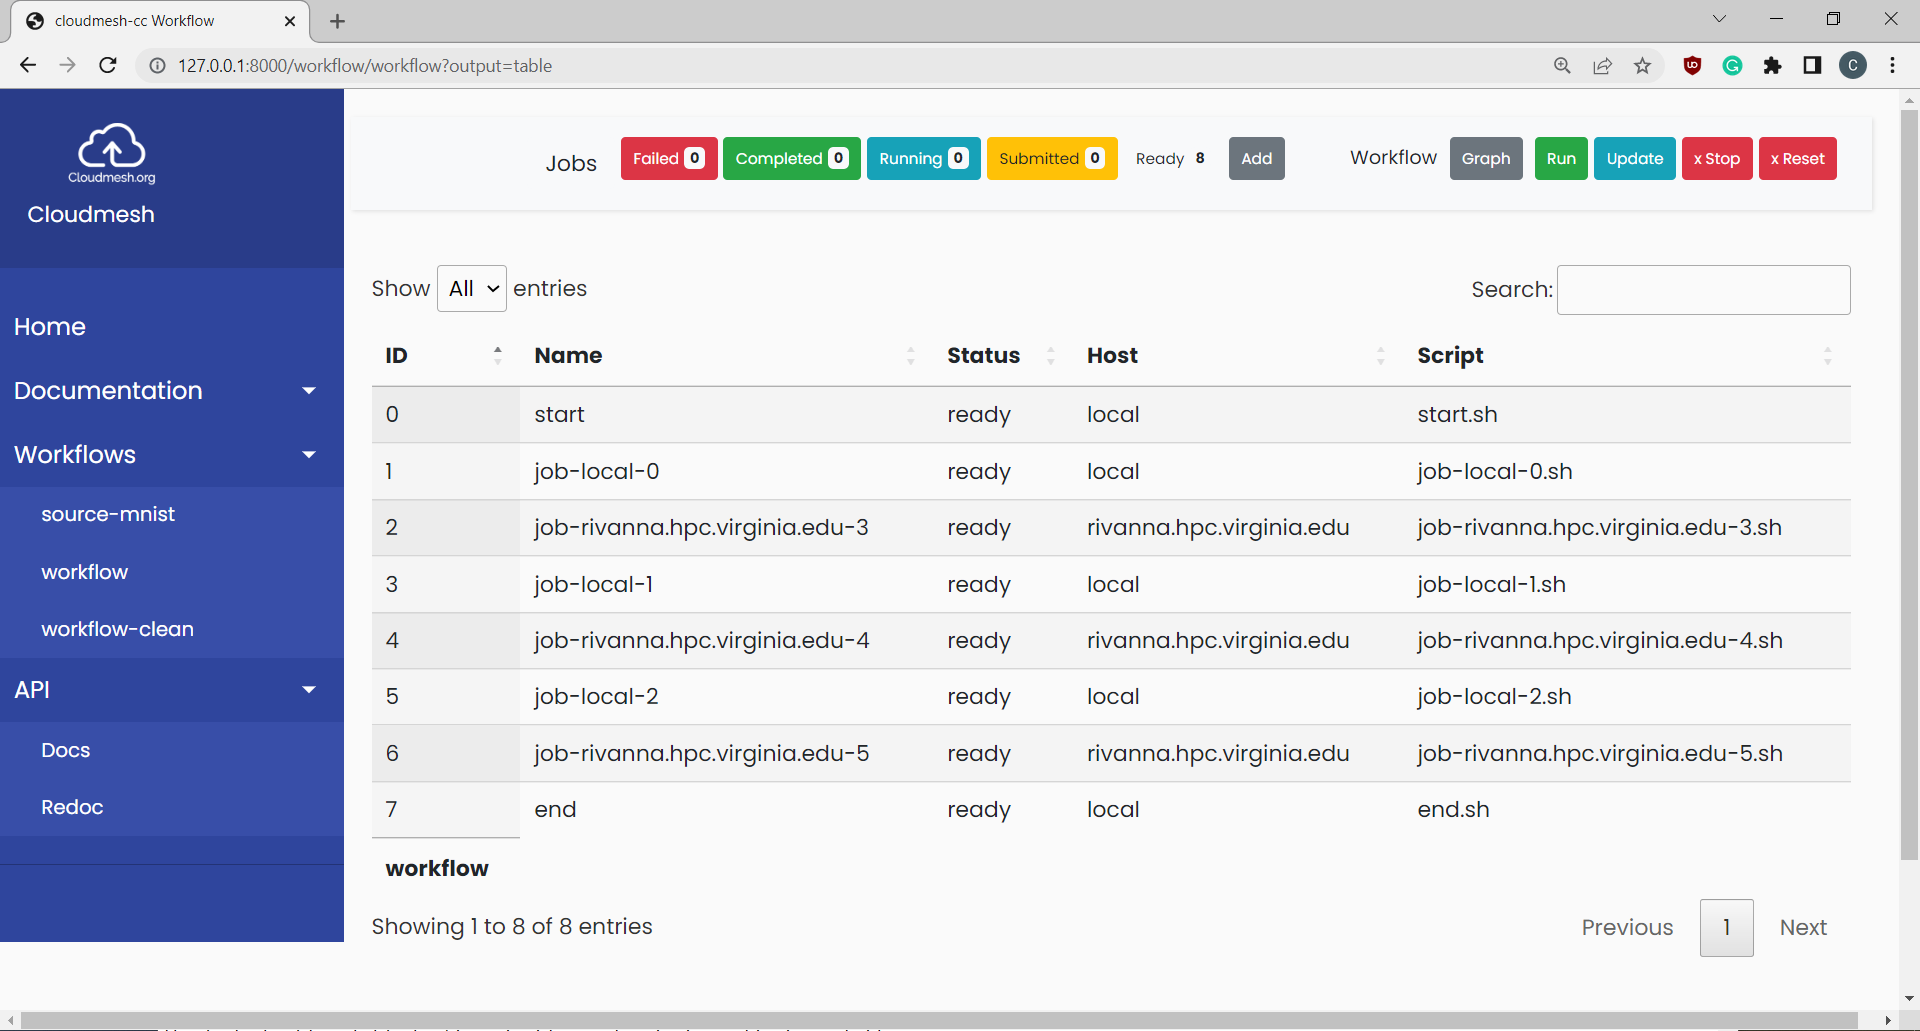
\includegraphics[width=1.0\columnwidth]{images/cc-1.png}
    \caption{Workflow user interface.}\label{fig:cc-3}
\end{figure}

We have tested the framework while running various MNIST application examples, including include Multilayer Perceptron, LSTM (Long short-term memory), Auto-Encoder, Convolutional, and Recurrent Neural Networks, Distributed Training, and PyTorch training. 
A much larger application using earthquake prediction has also been used.

Figure \ref{fig:fastapi-cc-arch} shows the REST specification and Figure \ref{fig:cc-2} shows the architecture. A user interface of the running application is shown in Figure \ref{fig:cc-3}.

% \subsubsection{Federated Analytics Service Catalogue}
% \subsubsection{Catalogue Attributes}
% \subsubsection{Federated analytics service Registries}
% \subsubsection{Registry Attributes}

% \subsection{Resource Accessibility}
% \subsubsection{Resource Management}
% \subsubsection{Security}



\FILE{section-data}
\subsection{Data Management}
\label{sec:data}

Managing data in analytics services is an important implicit
requirement. THe data has to be readily accessible and may have to be
prestaged to the resources where the computation is performed. ALso
one has to make sure that policy restrictions are appropriately dealt
with in order to perform the analytics tasks. The policy restrictions
typically include the total sze of the data for a particular user or
group, but also could include the number of files.

For this reason it is advantageous to have aservice that can deal with
such restrictions. Unfortunately such services are not readily
available based on our experience with different HPC centers offering
compute resources for analytics tasks and jobs.

Available services are typically restricted to filesystems that are
accessible on the compute nodes as well as services that copy between
local computers or between compute centers. The later is is frequently
covered by `rsync` over SSH or UDP, or through
Globus \cite{www-globus-transfer} as a service. However, when we tried
using Globus we found that it is not usable when millions of iles are
involved, but performs well when in such cases a tar file is produced
over amny files and the tar fle is transfered in a single
operation. We also encountered frequent timeouts on the servers that
were involved in a server-server transfer useing many file transfers.

To simplify this we developed a program
cloudmesh-globus \cite{cloudmesh-globus} that allows us to specify an
entire directory with many files that first automatically packages the
directory and transfers the compressed file to the remote machine
where it than gets uncompressed and placed in the appropriate file
ssytem. Hence such steps have not to be done by hand by the
researcher, but are done automated providing a simplified
filesystem-to-filesystem service via Globus without issues.

Other alternatives could include
cloudmesh-storage \cite{cloudmesh-storage} which include prototype
transfer services even among cloud providers such as amazon, azure,
and google, while leveraging a compute services conductiong file
copies between the involved parties.




\FILE{section-package.tex}

\subsection{Package Analytic Algorithms as Service Payloads}
\label{sec:package}

Here we explore how to package analytic algorithms with well-defined
input and output parameters as service payloads that can be reusable,
deployable, and operational across multi-cores, CPUs, and GPU
computing platforms.




\FILE{section-interfaces.tex}

\subsection{Analytics Interfaces}
\label{sec:interfaces}



\section{Resource Management}
\label{sec:resources}

Here we investigate and define a minimal set of resource management
services and interfaces for application orchestration and workflow
between processes.


\FILE{section-security.tex}

\section{Security}
\label{sec:security}

\subsection{Artifacts}

function
data
logs / audit

\subsection{Privacy}

privacy
    input
    output
    function
    
asynchronous events, how does privacy apply
batch functions
streaming functions

data


\subsection{Federation}

NIST document on federation

\subsection{Authentication}

\subsection{Authorization}

\subsection{Potential role of blockchain}


% \FILE{section/nlp.tex}

\subsection{NLP}


Natural Language Processing is one of the first services offored by
many cloud providers. THis is motivated by analyzing large amounts of
text in volume and number and deriving automated content from
it. Populare services include keyword extratction, sentiment analysis,
auto summary, and translation.  The services are offerd often by large
cloud providers such as Google, IBM Watson and Amazon to consumers for
a fee. In addition such tools are also offered as stand alone
components and software packages.

As many such services are offered by the different providers, and
standalone components and software packages exist, it allows us to use
them to test the framework for implementing hybrid and multi-cloud
analytics services. We can therefore analyze each of their APIs and
compare functionality as well as the perfomance charactaristics of
local as well as cloudservices. We also can test our design of the
cloud service catalog to identify the strategy of dynamically
loacating similar services and integrate them into a service offering.

For our work we have restricted our analysis to two cloud services
from Amazon ans Google, while the integration of a third from Amazon
is under development. Furthermore we have only considered the
translation service as it provides an easy abstraction of a service
that translates a text from a source language to a target langauge:

\begin{Verbatim}[fontsize=\small]
def translate(text, source_langauge, target_langauage, ...):
    ...
    return translation
\end{Verbatim}

Each of the services is implemented with a different API. We contrast
the API in Figure ... showcaseing the difference in invoking a
translation service as well as showcasing the result of the json
response of such a service.


If the interface is on purpose defined differently a switch will cost
extra work and may therfore not be in the interest of the users.  It
is obvious that users can benefit from a uniform implementation of
this API in order to easily switch from one provider to the other.
Naturally the cloud providers typically do not have any interrest in
providing such a uniform API as it may entise the customers to switch
service providers.

Hence a multicloud CLI implementation may look as followes, where the
provider flag is used to distinguish the different cloud providers
offering the translation service. Naturally, we could also utilize a
local translation program such as offered from ... and easily make
this example a hybrid service that also integrates with a local
implementation.

%\resizebox{1.0\columnwidth}{!}{
\begin{Verbatim}[fontsize=\small]
cms nlp translate --provider=google --from=en --to=de hello world
cms nlp translate --provider=aws --from=en --to=de hello world
cms nlp translate --provider=local --from=en --to=de hello world
\end{Verbatim}
%}


As eachof the services returns natively a different outout, it is
beneficial to unify the output and create a mapping from the
originating service to the output. An example for such a uniform output is given next.


\begin{Verbatim}[fontsize=\small]
{'date': '05/02/2022 14:45:45',
 'input': 'hello world',
 'input_language': 'en',
 'output': 'Hallo Welt',
 'output_language': 'de',
 'provider': 'aws',
 'time': 0.2641}
\end{Verbatim}


Other parameters such as service region can easily be integrated in
this example. Furthermore, it is obvious that the commandline
application underlaying API can be used in a REST service
implementation and can be generalized into different REST service
frameworks. For our implementation we have used FastAPI and used the
closest regional service center to our location.

The result of the translation that simply translates a text from
German ``Hallo Welt'' to English ``Hello World'' is showcased for 100
invocations in Figure~\ref{fig:translate}. 


\begin{figure}[htb]

\centering
%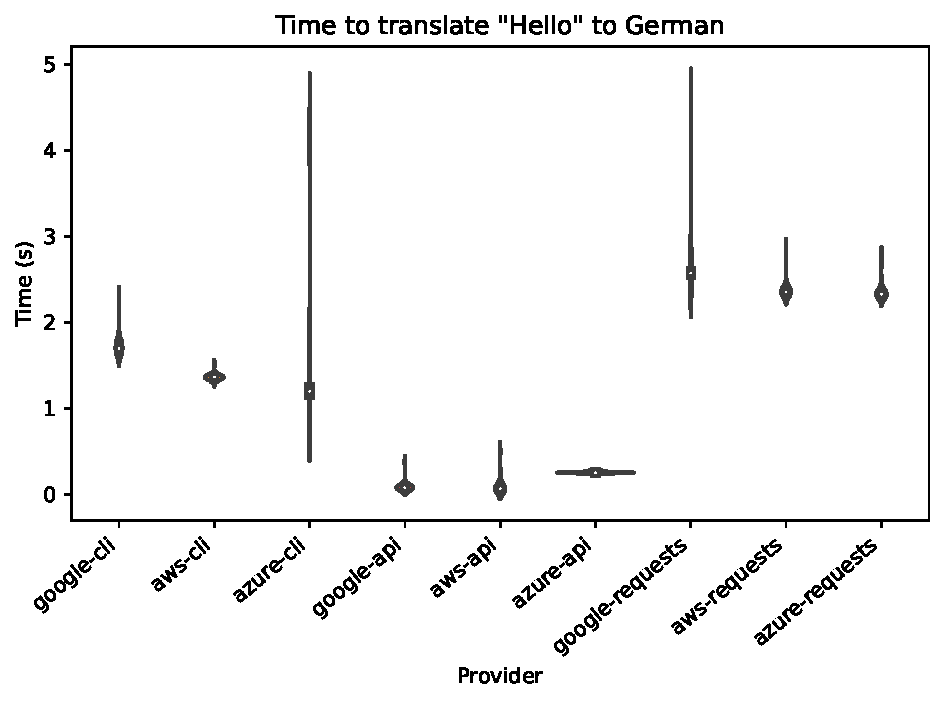
\includegraphics{images/nlp-benchmark.pdf}
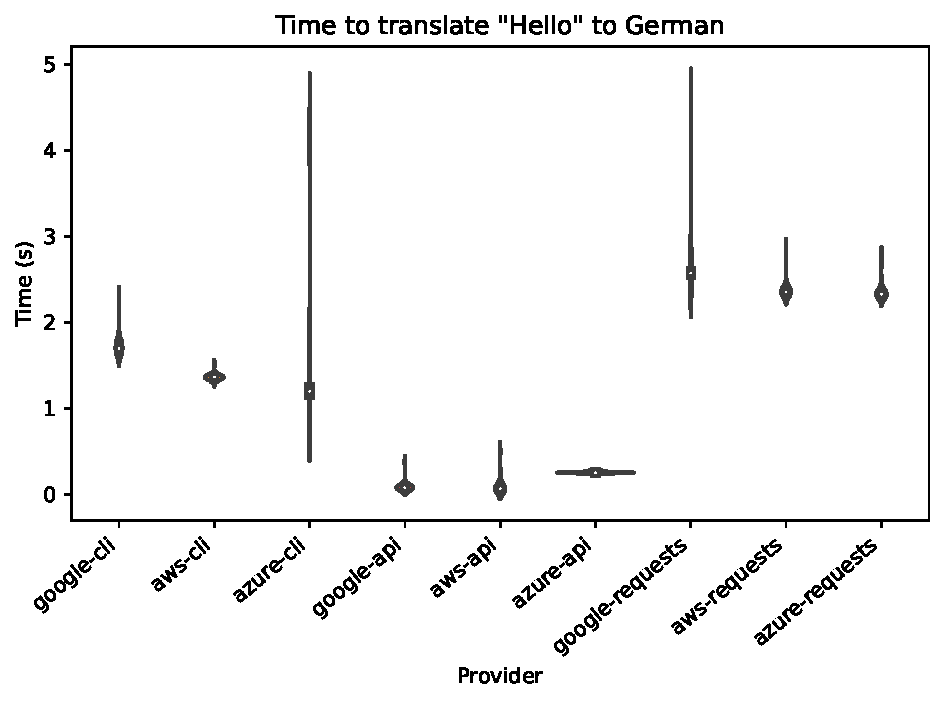
\includegraphics[width=1.0\columnwidth]{images/nlp-benchmark.pdf}

\caption{Natural Languge processing performance for a single
         word translation.}
\label{fig:nlp-performance}

\end{figure}


Such a performance analysis could be performed based on customer needs
and could indicate factors for preferential service choices. THis may
include besides time other factors such as cost and qaulity, or even
service level reliability at different times.

For us we found that in for the short query we used the service
offered by AWS to translate the text was on average ...  seconds
faster when executed from Bloomington, IN to the closest service
centers for the providor.


\begin{table*}[htb]

\caption{Comparision of the time it takes on average to translate the word hello from English to German}

\begin{tabular}{lrrrrrrrrr}
 & google-cli & aws-cli & azure-cli & google-api & aws-api & azure-api & google-requests & aws-requests & azure-requests \\
 \hline
count & 20.000000 & 20.000000 & 20.000000 & 20.000000 & 20.000000 & 20.000000 & 20.000000 & 20.000000 & 20.000000 \\
mean & 1.737850 & 1.369900 & 1.365600 & 0.094800 & 0.099300 & 0.257150 & 2.681500 & 2.381500 & 2.352550 \\
std & 0.134381 & 0.043240 & 0.664569 & 0.066135 & 0.104365 & 0.009292 & 0.429593 & 0.111200 & 0.100339 \\
min & 1.643000 & 1.297000 & 1.120000 & 0.069000 & 0.064000 & 0.245000 & 2.532000 & 2.330000 & 2.299000 \\
25\% & 1.675250 & 1.346750 & 1.162750 & 0.075000 & 0.066750 & 0.251000 & 2.556750 & 2.349250 & 2.316500 \\
50\% & 1.695000 & 1.366500 & 1.198500 & 0.079000 & 0.067500 & 0.255000 & 2.574000 & 2.354000 & 2.329500 \\
75\% & 1.749000 & 1.378750 & 1.246750 & 0.085750 & 0.069250 & 0.259500 & 2.592750 & 2.367750 & 2.341500 \\
max & 2.266000 & 1.520000 & 4.170000 & 0.374000 & 0.497000 & 0.280000 & 4.481000 & 2.848000 & 2.766000 \\
\hline
\end{tabular}
\end{table*}

/clearpage


% \section{Conclusion}

In this paper, we have outlined our thoughts on building an analytics services framework. We have integrated aspects to make these services hybrid services across various compute providers including HPC, clouds, and microservices.

In addition to this exploratory thought, a component-based prototype implementation leveraging cloudmesh has been used to verify the feasibility of the approach. It has then been tested theoretically on some applications, while it also has been practically explored in the area of natural language processing and earthquake forecasting.

Furthermore, the framework has been used intensely as part of the MLCommons Science Working group where it was used for additional application.


\bibliographystyle{ACM-Reference-Format}
\bibliography{NIST-analytics}

% \appendix

%\FILE{section-glossary.tex}

\section{Glossary}
\label{sec:glossary}

THis Glossary provides terms that aur used in this document. In
addition we have provided a definitions in Section \ref{sec:defining}
to focus on the details of some terms and terminology used in this
document specifically focussing on Analytics Servoces.

\begin{description}

  
\item[AAI:] Authentication and Authorization
  Infrastructure. Facilitates single, virtualized identities (issued
  by the {\em user’s home organization.})

\item[AARC:]   \TODO{Russell}{The Authentication and Authorisation for
  Research and Collaboration project. I will write a descriptive
  sentence for it that you can add later. Also, below, ACL: access
  control list? I have a bunch other acronyms with descriptions that I
  can just send you as a list that you can choose from and add if you
  wish. Under Iaas, p is probably referring to PaaS}  

\item[ABAC:] attribute based access control

\item[ACL:] \TODO{Russell}{TBD}

\item[ACID:] Atomicity, Consistency, Isolation, Durability.

\item[Analytics:] The systematic analysis of data, to uncover patterns
  and relationships between data, historical trends, and attempts at
  predictions of future behaviors and events.

\item[Analytics management:] A sub function within the [metadata]
  registry.

\item[Analytics services] azure cognitive, google analytics, aws
  [dozens], watson analytics... in contrast to ML frameworks like
  tensorflow, pytorch, caffe2, and in contrast to Programming
  libraries like python, scikit, shiny, or R Studio [??]


\item[Analytics Workflow:] The sequence of processes or tasks part of
  the analysis

\item[API:] Application Programming Interface

\item[ASCII:] American Standard Code for Information Interchange

\item[BASE:] Basically Available, Soft state, Eventual consistency
  Classification scheme per 11179, a container of the classifiers for
  all kinds of administered items including common data elements
  [CDE]s.

\item[CIA:] Confidentiality, Integrity, and Availability.

\item[CLI:] Command Line Interface.

\item[Consumer:] Ametadata consumer, per IHE, is responsible for the
  import of metadata created by the source. In the context of section
  A.3,

\item[Container:] See
  \url{http://csrc.nist.gov/publications/drafts/800-180/sp800-180_draft.pdf}
  Cloud Computing The practice of using a network of remote servers
  hosted on the Internet to store, manage, and process data, rather
  than a local server or a personal computer. See
  \url{http://nvlpubs.nist.gov/nistpubs/Legacy/SP/nistspecialpublication800-145.pdf}.

\item[CDE:] Common data element = smallest meaningful data container
  in a given context.

\item[DDC:] data dictionary component. library of data elements that
  are used to establish common understanding of the meaning of coding
  systems.

\item[Data element:] Describes [or defines] the logical unit of
  data. Per 11179, the element refers to the structure of the data,
  distinct from a data instance.

\item[Data element concept:] the combination of an object class, and a
  related property.

\item[DEX:] Data element exchange = interoperability profile. Enables
  retrieval of extraction specifications for data elements which are
  defined in particular domains. “Options” including the cross
  enterprise doc sharing [XDS] doc type binding option and the cross
  community access [XCA] doc type binding option, extend basic DEX
  functionality, addressing interoperability with Secondary Data
  Usage[s]. Allowing secondary users to know if and where [data] is
  available when it is organized as a doc sharing environment,
  I.e. XDS, MPQ, XCA.

\item[DevOps:] A clipped compound [?] [portmanteau?] of software
  DEVelopment and information technology OPerationS \TOFO{{}{improve}

\item[Deployment:] The action of installing software on resources

\item[DMTF:] Distributed Management Task Force. A standards
  organization.

\item[Extraction Specification:] a map of data locations used as a
  guide for extracting data. SPARQL, SQL, and XPath scripts, aka
  mapping scripts, are examples of specifications for locating a data
  element in a particular content model.

\item[FIM:] federated identity management. A core component of AAI.


\item[Federated database system:] two definitions: 1. a system that
  maps multiple autonomous database systems using a combining scheme
  where one DB interface is provided for local / owner access to data,
  and another simpler interface is provided for guest access to non
  owner data. 2. a DBMS which is an element of a federated group, that
    allows members belonging to the same federated group, to access
    data residing in the DBMS.

\item[HTTP:] HyperText Transfer Protocol HTTPS HTTP Secure

\item[Hybrid Cloud:] See
  \url{http://nvlpubs.nist.gov/nistpubs/Legacy/SP/nistspecialpublication800-145.pdf}.


\item[IaaS:] Infrastructure as a Service SaaS Software as a Service
  Implementation.

\item[IGTF:] Interoperable Global Trust Federation.

\item[ITL:] Information Technology Laboratory metadata data employed
  to annotate other data with descriptive information.

\item[IHE:} \TODO{russel}{TBD}

\item[LDAP:] Lightweight Directory Access Protocol. A
  directory/registry standard.

\item[Metadata generator:] A sub function within the repository
  Metadata Registry [MDR] a database that manages the semantics of
  data elements, and this case, provides discovery and analytics
  management services.

\item[MRR:] Metadata registry / repository = specialized DB of
  metadata which describe data constructs.

\item[Microservice:] Architecture Is an approach to build applications
  based on many smaller modular services. Each module supports a
  specific goal and uses a simple, well-defined interface to
  communicate with other sets of services.

\item[NBDIF] \TODO{}{TBD}
  
\item[NBD-PWG:] NIST Big Data Public Working Group.

\item[NBDRA:] NIST Big Data Reference Architecture.

\item[NBDRAI:] NIST Big Data Reference Architecture Interface.

\item[NIEM:] National information exchange model = government wide
  standards based approach to exchanging information in the US.

\item[NIST:] National Institute of Standards and Technology.

\item[OGF:] Open Grid Forum.

\item[OS:] Operating System.

\item[P2P:] Peer to Peer.

\item[PKI:] Public Key Infrastructure. a security related certificate
  aka X.509.

\item[Proxy:] \TODO{}{TBD}

\item[Registry:] \TODO{}{TBD}
  
\item[Registry, federated:] \TODO{}{TBD}


\item[REST:] REpresentational State Transfer Retrieval a transaction
  where a system returns a selection I.e. a list of data elements from
  a database, or in the scope of this document, a list of elements in
  a metadata registry.

\item[SAML:] Security assertion markup language. a security standard;
  web browser service that defines “syntax and semantics to exchange
  auth and auth data between security domains.” Not compatible with
  other authentication protocols such as Secure socket?, OIDC, etc.

\item[Serverless Computing:] Serverless computing specifies the
  paradigm of function as a service (FaaS). It is a cloud computing
  code execution model in which a cloud provider manages the function
  deployment and utilization while clients can utilize them. The
  charge model is based on execution of the function rather than the
  cost to manage and host the VM or container.

\item[Services:] \TODO{}{TBD}

\item[Service registry:] in the context of an SOA architecture, this
  registry is a network based directory that contains available
  services.

\item[Software stack:] A set of programs and services that are
  installed on a resource to support applications.  Value domain the
  description of a permissible set of values for the property of a
  data element definition.

\item[XACML] eXtensible Access Control Markup Language. a security
  related standard developed by OASIS, circa 2005.

\end{description}




\end{document}
\endinput
%%%%%%%%%%%%%%%%%%%%%%%%%%%%%%%%%%%%%%%%%%%%%%%%%%%%%%%%%%%%%%

